%!TEX root = lot2.tex

%--------------------------CARTES NEUTRE------------------------------------------------------------------------------------------------

\begin{tikzpicture} %Recto
	%Fond
    \node[anchor=south west,inner sep=0] (carte) at (0,0) {
\includegraphics[width=7.1 cm, height=9.6 cm]{fonds/noir.png}};
    \node[anchor=center] at (carte.center) {
\includegraphics[width=\cardwidth cm, height=\cardheight cm]{fonds/fond_plan.png}};
\end{tikzpicture}

\begin{tikzpicture} %Verso
	%Fond
    \node[anchor=south west,inner sep=0] (carte) at (0,0) {
\includegraphics[width=7.1 cm, height=9.6 cm]{fonds/noir.png}};
    \node[anchor=center] at (carte.center) {
\includegraphics[width=\cardwidth cm, height=\cardheight cm]{fonds/fond_plan.png}};
\end{tikzpicture}

\begin{tikzpicture} %Recto
	%Fond
    \node[anchor=south west,inner sep=0] (carte) at (0,0) {
\includegraphics[width=7.1 cm, height=9.6 cm]{fonds/noir.png}};
    \node[anchor=center] at (carte.center) {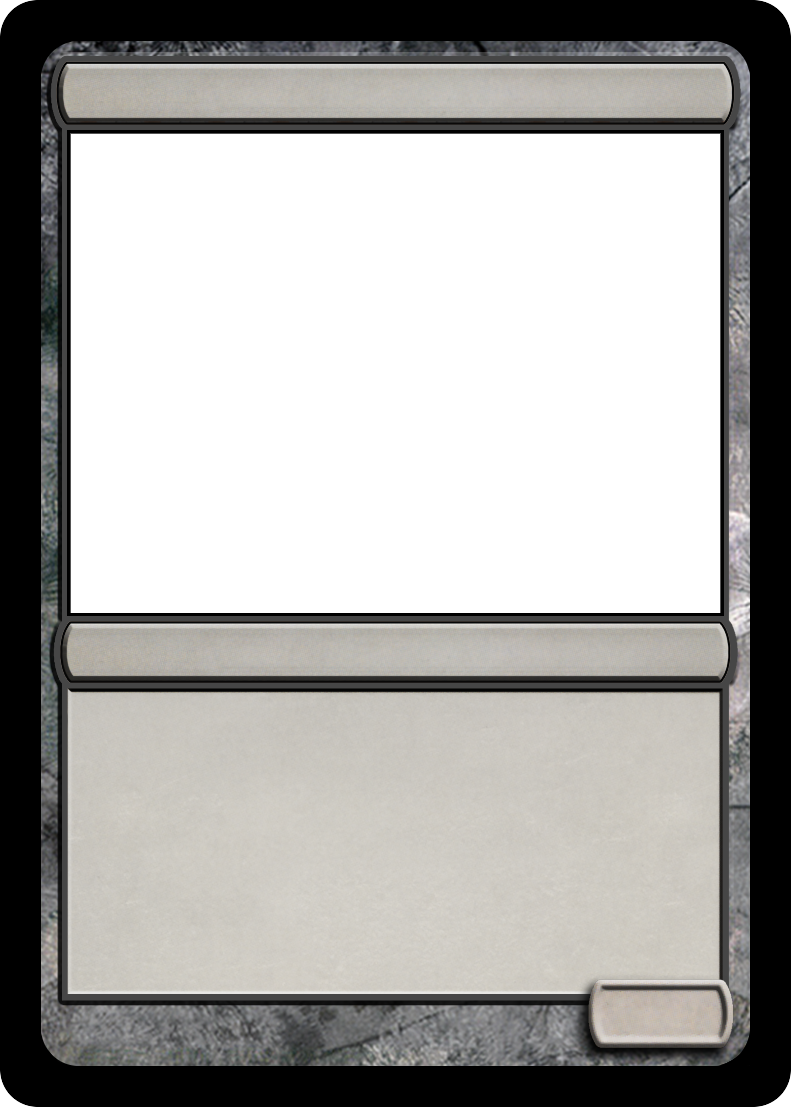
\includegraphics[width=\cardwidth cm, height=\cardheight cm]{fonds/fond_neutre.png}};

    %Titre
	\node[anchor=center] at (\titleX,\titleY) {\titlefont Ambition Boost};

	%Image
	\node[anchor=center] at (\imageX,\imageY) {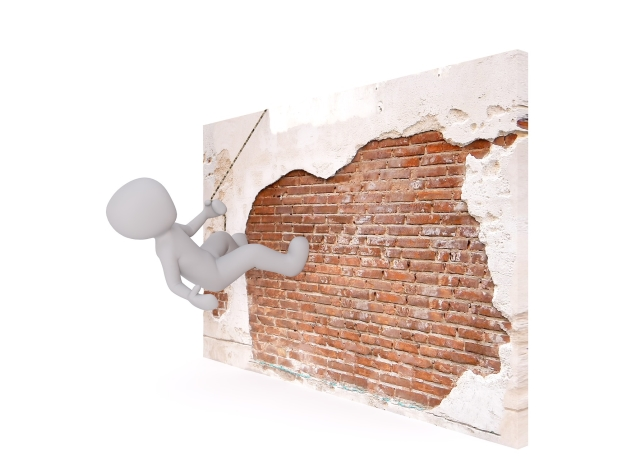
\includegraphics[width=\imageWidth px, height=\imageHeight px]{images/UO_50_ambition.jpg}};
	\node[anchor=center] at (6.1,4.5) {
\includegraphics[width=12 px, height=6 px]{fonds2/legacy.jpg}};

	%Type
	\node[anchor=center] at (\typeX,\typeY) {\typefont Neutre};

	%Description
	\node[anchor=north west, text width=5.6cm] (description) at (\descriptionX,\descriptionY) {\descriptionfont\setsize{8}Chaque autre joueur invente une phrase de winner. En tant que leader Ambition Boost, vous et le winner que vous désignez défaussez une carte.\par};

	%Punchline
	\node[anchor=north west, text width=5.6cm, below = 1pt of description] (punchline) {\punchlinefont\setsize{8}``Tout obstacle renforce la détermination. Celui qui s’est fixé un but n’en change pas.''\par};

	%Separateur !!!!!PAS TOUCHE!!!!!
	\fill[black,path fading=west] (description.south west) rectangle (punchline.north);
	\fill[black,path fading=east] (punchline.north) rectangle (description.south east);

	%Numéro !!!!!PAS TOUCHE!!!!!
	\node[anchor=center] at (\numberX,\numberY) {\numberfont \cardnumber};
\end{tikzpicture}\verso %Verso


\begin{tikzpicture} %Recto
	%Fond
    \node[anchor=south west,inner sep=0] (carte) at (0,0) {
\includegraphics[width=7.1 cm, height=9.6 cm]{fonds/noir.png}};
    \node[anchor=center] at (carte.center) {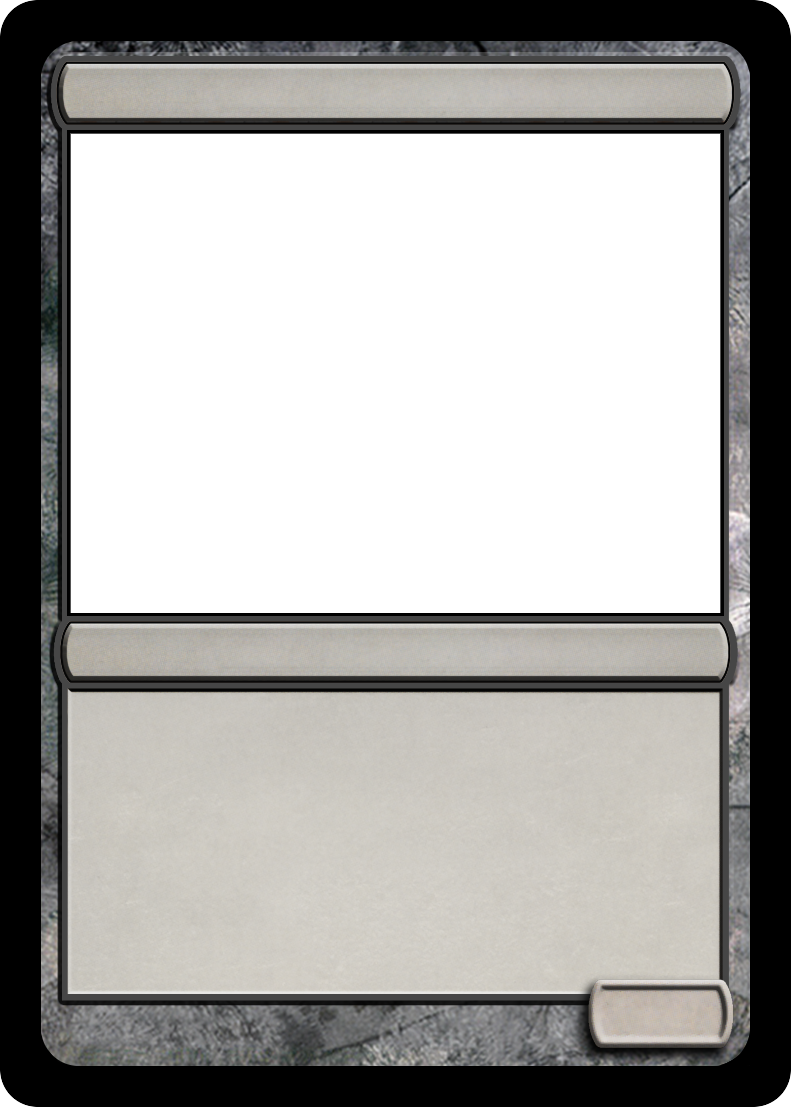
\includegraphics[width=\cardwidth cm, height=\cardheight cm]{fonds/fond_neutre.png}};

    %Titre
	\node[anchor=center] at (\titleX,\titleY) {\titlefont Man in the Middle};

	%Image
	\node[anchor=center] at (\imageX,\imageY) {
\includegraphics[width=\imageWidth px, height=\imageHeight px]{images/UO_39_Middle.jpg}};
	\node[anchor=center] at (6.1,4.5) {
\includegraphics[width=12 px, height=6 px]{fonds2/legacy.jpg}};

	%Type
	\node[anchor=center] at (\typeX,\typeY) {\typefont Neutre (Interruption)};

	%Description
	\node[anchor=north west, text width=5.6cm] (description) at (\descriptionX,\descriptionY) {\descriptionfont\setsize{8}A tout moment vous pouvez jouer cette carte pour jouer une carte à la place d’un autre joueur.\par};

	%Punchline
	\node[anchor=north west, text width=5.6cm, below = 1pt of description] (punchline) {\punchlinefont\setsize{8}On vous avait bien dit que 16 bits de MAC étaient insuffisants.\par};

	%Separateur !!!!!PAS TOUCHE!!!!!
	\fill[black,path fading=west] (description.south west) rectangle (punchline.north);
	\fill[black,path fading=east] (punchline.north) rectangle (description.south east);

	%Numéro !!!!!PAS TOUCHE!!!!!
	\node[anchor=center] at (\numberX,\numberY) {\numberfont \cardnumber};
\end{tikzpicture}\verso %Verso

\begin{tikzpicture} %Recto
	%Fond
    \node[anchor=south west,inner sep=0] (carte) at (0,0) {
\includegraphics[width=7.1 cm, height=9.6 cm]{fonds/noir.png}};
    \node[anchor=center] at (carte.center) {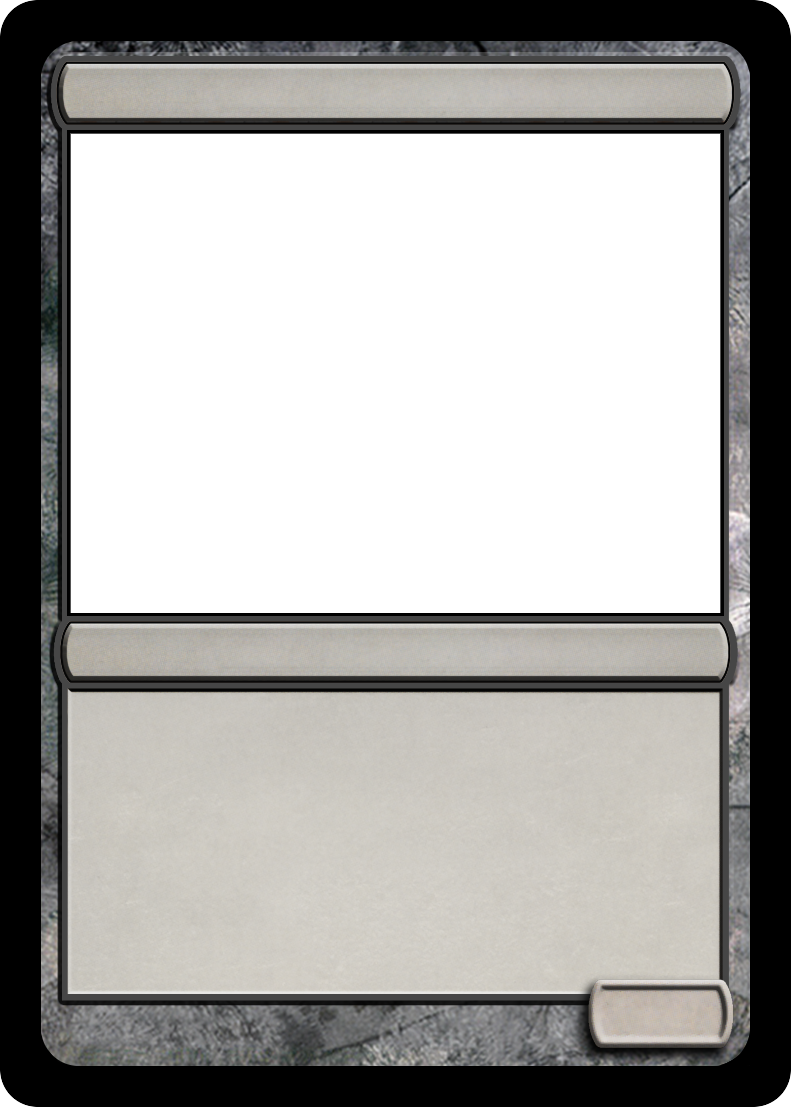
\includegraphics[width=\cardwidth cm, height=\cardheight cm]{fonds/fond_neutre.png}};

    %Titre
	\node[anchor=center] at (\titleX,\titleY) {\titlefont Blague lourde de votre manager};

	%Image
	\node[anchor=center] at (\imageX,\imageY) {
\includegraphics[width=\imageWidth px, height=\imageHeight px]{images/UO_45_sexe.jpg}};
	\node[anchor=center] at (6.1,4.5) {
\includegraphics[width=12 px, height=6 px]{fonds2/legacy.jpg}};

	%Type
	\node[anchor=center] at (\typeX,\typeY) {\typefont Neutre};

	%Description
	\node[anchor=north west, text width=5.6cm] (description) at (\descriptionX,\descriptionY) {\descriptionfont\setsize{8}Ça n’a aucun effet mais vous vous sentez profondément humilié. Le manager doit raconter une blague.\par};

	%Punchline
	\node[anchor=north west, text width=5.6cm, below = 1pt of description] (punchline) {\punchlinefont\setsize{10}``Vous n’avez pas de sexe.''\par};

	%Separateur !!!!!PAS TOUCHE!!!!!
	\fill[black,path fading=west] (description.south west) rectangle (punchline.north);
	\fill[black,path fading=east] (punchline.north) rectangle (description.south east);

	%Numéro !!!!!PAS TOUCHE!!!!!
	\node[anchor=center] at (\numberX,\numberY) {\numberfont \cardnumber};
\end{tikzpicture}\verso %Verso


\begin{tikzpicture} %Recto
	%Fond
    \node[anchor=south west,inner sep=0] (carte) at (0,0) {
\includegraphics[width=7.1 cm, height=9.6 cm]{fonds/noir.png}};
    \node[anchor=center] at (carte.center) {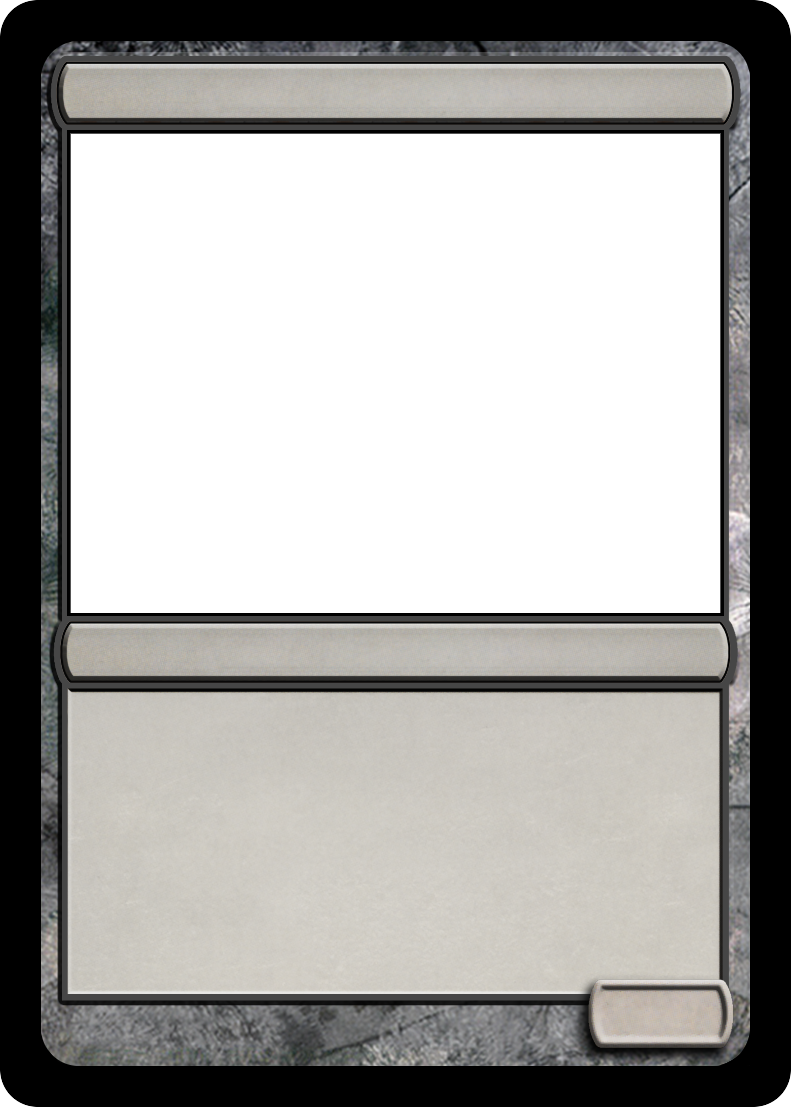
\includegraphics[width=\cardwidth cm, height=\cardheight cm]{fonds/fond_neutre.png}};

    %Titre
	\node[anchor=center] at (\titleX,\titleY) {\titlefont SVN cassé};

	%Image
	\node[anchor=center] at (\imageX,\imageY) {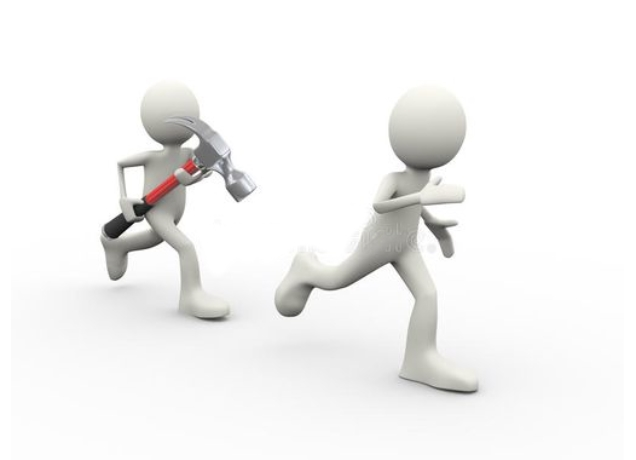
\includegraphics[width=\imageWidth px, height=\imageHeight px]{images/SVN.jpg}};
	\node[anchor=center] at (6.1,4.5) {
\includegraphics[width=12 px, height=6 px]{fonds2/legacy.jpg}};

	%Type
	\node[anchor=center] at (\typeX,\typeY) {\typefont Neutre};

	%Description
	\node[anchor=north west, text width=5.6cm] (description) at (\descriptionX,\descriptionY) {\descriptionfont\setsize{8}Faites un tirage aléatoire pour retrouver le coupable. Ce dernier pioche une carte.\par};

	%Punchline
	\node[anchor=north west, text width=5.6cm, below = 1pt of description] (punchline) {\punchlinefont\setsize{8}``Qui a encore choucrouté le SVN ?@!!!''\\-Obi\par};

	%Separateur !!!!!PAS TOUCHE!!!!!
	\fill[black,path fading=west] (description.south west) rectangle (punchline.north);
	\fill[black,path fading=east] (punchline.north) rectangle (description.south east);

	%Numéro !!!!!PAS TOUCHE!!!!!
	\node[anchor=center] at (\numberX,\numberY) {\numberfont \cardnumber};
\end{tikzpicture}\verso %Verso

\begin{tikzpicture} %Recto
	%Fond
    \node[anchor=south west,inner sep=0] (carte) at (0,0) {
\includegraphics[width=7.1 cm, height=9.6 cm]{fonds/noir.png}};
    \node[anchor=center] at (carte.center) {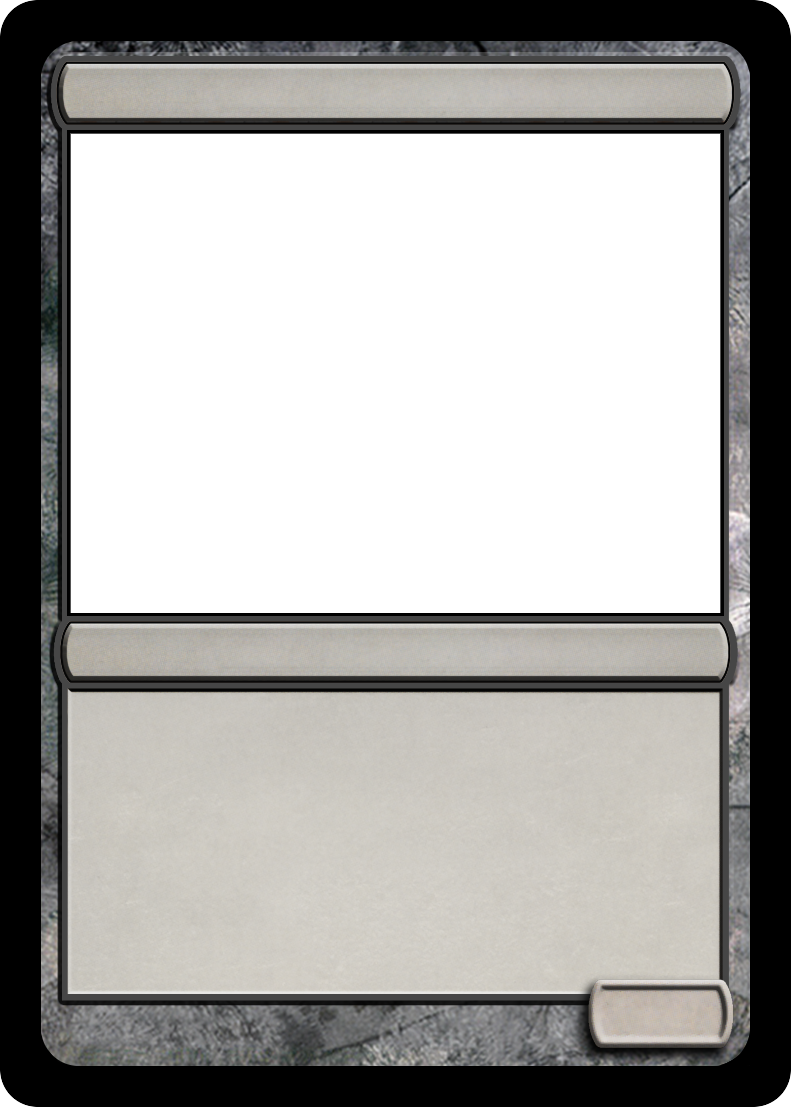
\includegraphics[width=\cardwidth cm, height=\cardheight cm]{fonds/fond_neutre.png}};

    %Titre
	\node[anchor=center] at (\titleX,\titleY) {\titlefont Random est une pute};

	%Image
	\node[anchor=center] at (\imageX,\imageY) {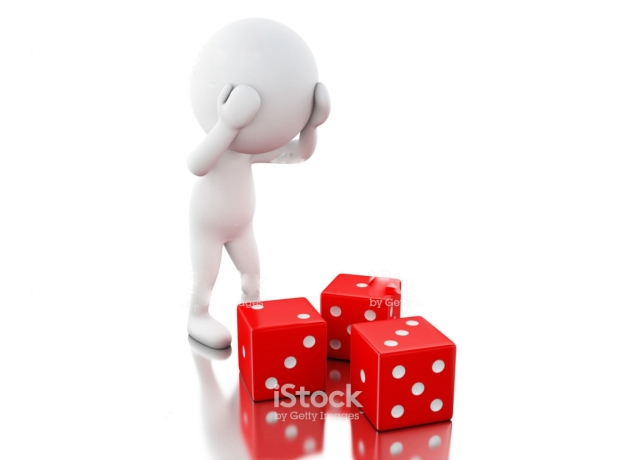
\includegraphics[width=\imageWidth px, height=\imageHeight px]{images/randompute.jpg}};
	\node[anchor=center] at (6.1,4.5) {
\includegraphics[width=12 px, height=6 px]{fonds2/legacy.jpg}};

	%Type
	\node[anchor=center] at (\typeX,\typeY) {\typefont Neutre};

	%Description
	\node[anchor=north west, text width=5.6cm] (description) at (\descriptionX,\descriptionY) {\descriptionfont\setsize{8}Lorsque vous jouez cette carte, vous mélangez les cartes de personnage de ce tour, un autre joueur donne un nombre, le personnage au rôle correspondant paie la tournée de café (reçoit une carte de chaque autre joueur).\par};

	%Punchline
	\node[anchor=north west, text width=5.6cm, below = 1pt of description] (punchline) {\punchlinefont\setsize{8}``En partant du haut ou du bas?''\par};

	%Separateur !!!!!PAS TOUCHE!!!!!
	\fill[black,path fading=west] (description.south west) rectangle (punchline.north);
	\fill[black,path fading=east] (punchline.north) rectangle (description.south east);

	%Numéro !!!!!PAS TOUCHE!!!!!
	\node[anchor=center] at (\numberX,\numberY) {\numberfont \cardnumber};
\end{tikzpicture}\verso %Verso

%%%%%%%%%%%%%%%%%%%%%%%%%%%%%%%%%%%%%%%%%%%%%%%%%%%%%%%%%%%%%%%%%
\begin{tikzpicture} %Recto
	%Fond
    \node[anchor=south west,inner sep=0] (carte) at (0,0) {
\includegraphics[width=7.1 cm, height=9.6 cm]{fonds/noir.png}};
    \node[anchor=center] at (carte.center) {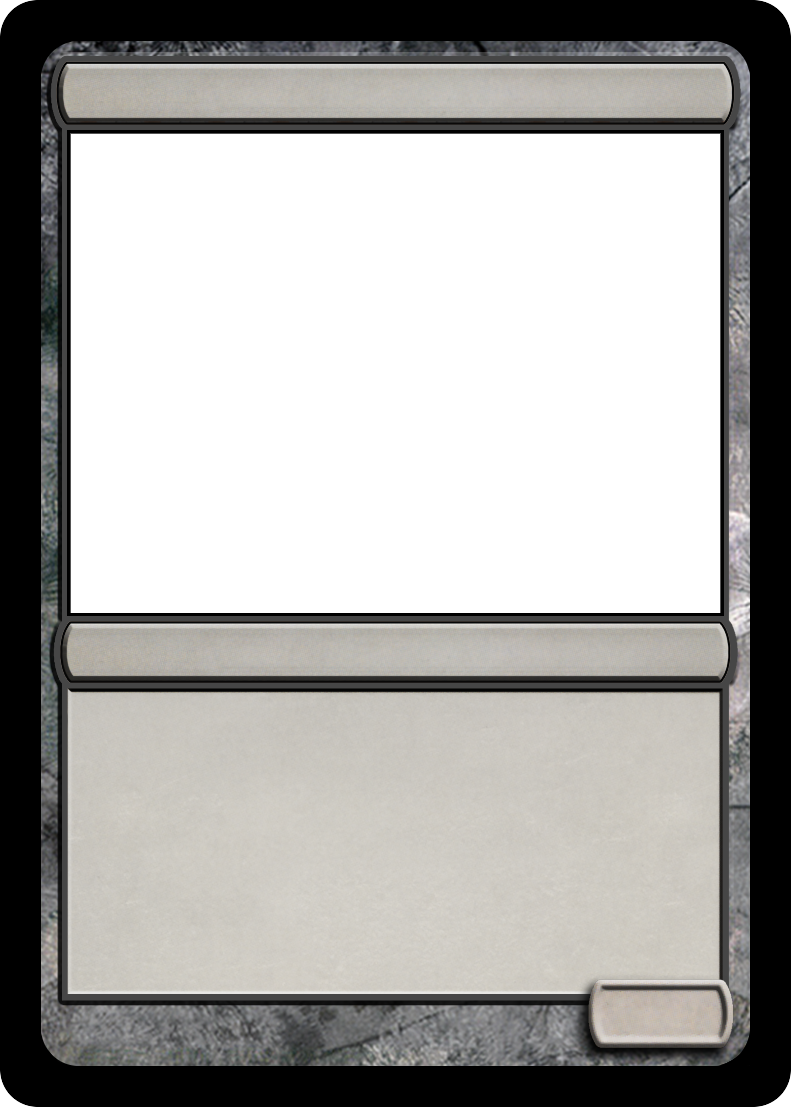
\includegraphics[width=\cardwidth cm, height=\cardheight cm]{fonds/fond_neutre.png}};

    %Titre
	\node[anchor=center] at (\titleX,\titleY) {\titlefont Gazette LCH};

	%Image
	\node[anchor=center] at (\imageX,\imageY) {
\includegraphics[width=\imageWidth px, height=\imageHeight px]{images/Gazette_LCH_v2.jpg}};
	\node[anchor=center] at (6.1,4.5) {
\includegraphics[width=12 px, height=6 px]{fonds2/legacy.jpg}};

	%Type
	\node[anchor=center] at (\typeX,\typeY) {\typefont Neutre};

	%Description
	\node[anchor=north west, text width=5.6cm] (description) at (\descriptionX,\descriptionY) {\descriptionfont\setsize{8}Chaque joueur doit nommer une carte que le joueur à sa gauche (néant si neutralisé) a joué le tour dernier. En cas d’erreur il pioche, si correct il défausse. Faites semblant d’écouter les autres joueurs comme tout le monde.\par};
	%Punchline
	\node[anchor=north west, text width=5.6cm, below = 1pt of description] (punchline) {\punchlinefont\setsize{8}``Petit tour de table, allô, Sylvain tu nous entend ?''\par};

	%Separateur !!!!!PAS TOUCHE!!!!!
	\fill[black,path fading=west] (description.south west) rectangle (punchline.north);
	\fill[black,path fading=east] (punchline.north) rectangle (description.south east);

	%Numéro !!!!!PAS TOUCHE!!!!!
	\node[anchor=center] at (\numberX,\numberY) {\numberfont \cardnumber};
\end{tikzpicture}\verso %Verso

%%%%%%%%%%%%%%%%%%%%%%%%%%%%%%%%%%%%%%%%%%%%%%%%%%%%%%%%%%%%%%%%%
\begin{tikzpicture} %Recto
	%Fond
    \node[anchor=south west,inner sep=0] (carte) at (0,0) {
\includegraphics[width=7.1 cm, height=9.6 cm]{fonds/noir.png}};
    \node[anchor=center] at (carte.center) {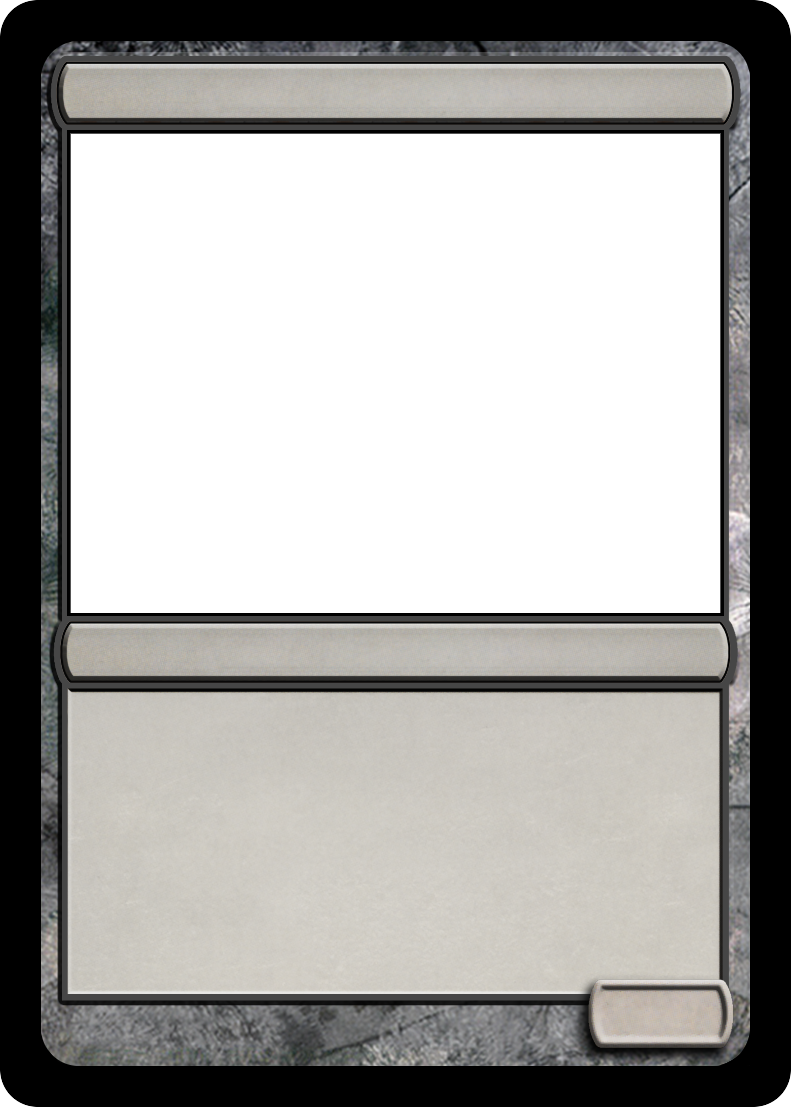
\includegraphics[width=\cardwidth cm, height=\cardheight cm]{fonds/fond_neutre.png}};

    %Titre
	\node[anchor=center] at (\titleX,\titleY) {\titlefont Un petit film ce week end ?};

	%Image
	\node[anchor=center] at (\imageX,\imageY) {
\includegraphics[width=\imageWidth px, height=\imageHeight px]{images/movie.jpg}};
	\node[anchor=center] at (6.1,4.5) {
\includegraphics[width=12 px, height=6 px]{fonds2/legacy.jpg}};

	%Type
	\node[anchor=center] at (\typeX,\typeY) {\typefont Neutre};

	%Description
	\node[anchor=north west, text width=5.6cm] (description) at (\descriptionX,\descriptionY) {\descriptionfont\setsize{8} Chaque autre joueur doit donner le titre d’un film sorti il y a moins d'un an ou piocher une carte.\par};
	
	%Punchline
	\node[anchor=north west, text width=5.6cm, below = 1pt of description] (punchline) {\punchlinefont\setsize{8} Ne lui dites surtout pas que vous détestez Interstellar.\par};

	%Separateur !!!!!PAS TOUCHE!!!!!
	\fill[black,path fading=west] (description.south west) rectangle (punchline.north);
	\fill[black,path fading=east] (punchline.north) rectangle (description.south east);

	%Numéro !!!!!PAS TOUCHE!!!!!
	\node[anchor=center] at (\numberX,\numberY) {\numberfont \cardnumber};
\end{tikzpicture}\verso %Verso

%%%%%%%%%%%%%%%%%%%%%%%%%%%%%%%%%%%%%%%%%%%%%%%%%%%%%%%%%%%%%%%%%
\begin{tikzpicture} %Recto
	%Fond
    \node[anchor=south west,inner sep=0] (carte) at (0,0) {
\includegraphics[width=7.1 cm, height=9.6 cm]{fonds/noir.png}};
    \node[anchor=center] at (carte.center) {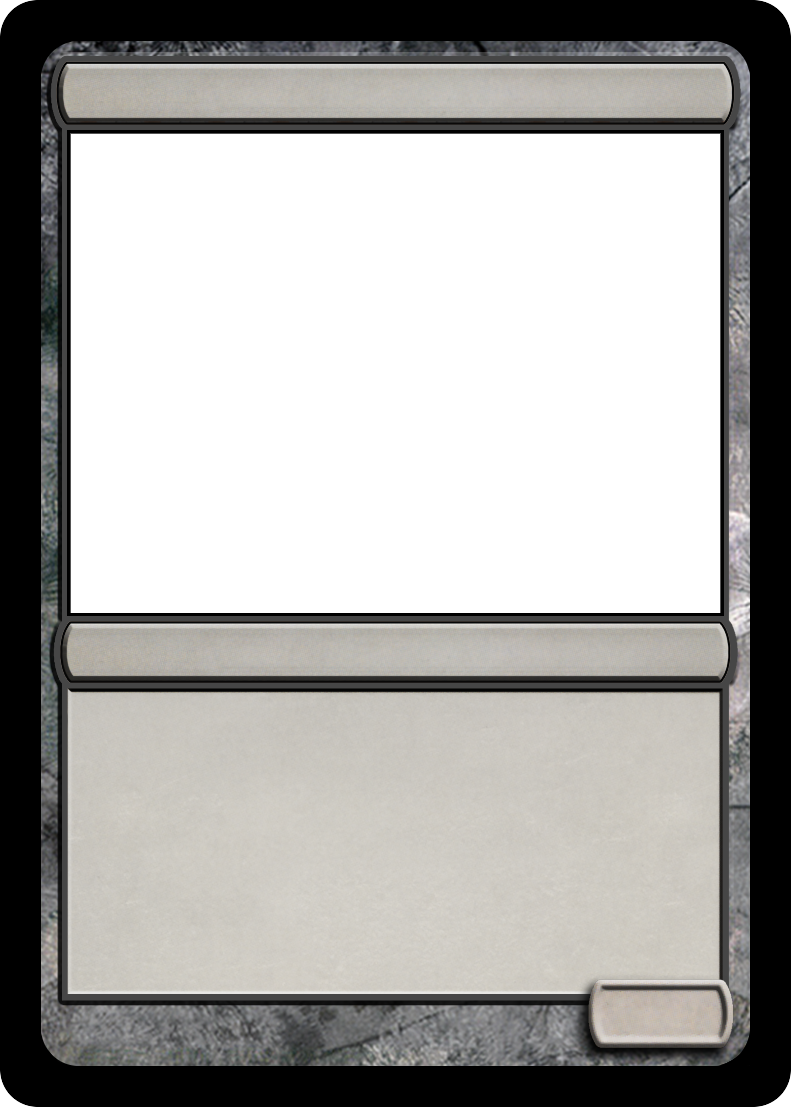
\includegraphics[width=\cardwidth cm, height=\cardheight cm]{fonds/fond_neutre.png}};

    %Titre
	\node[anchor=center] at (\titleX,\titleY) {\titlefont Mois de préavis};

	%Image
	\node[anchor=center] at (\imageX,\imageY) {
\includegraphics[width=\imageWidth px, height=\imageHeight px]{images/UO_45_preavis.jpg}};
	\node[anchor=center] at (6.1,4.5) {
\includegraphics[width=12 px, height=6 px]{fonds2/legacy.jpg}};

	%Type
	\node[anchor=center] at (\typeX,\typeY) {\typefont Neutre};

	%Description
	\node[anchor=north west, text width=5.6cm] (description) at (\descriptionX,\descriptionY) {\descriptionfont\setsize{6}Si la carte ANSSI est en jeu, vous pouvez immédiatement la faire pivoter d'un quart de tour, dans le sens que vous voulez. \par};

	%Numéro !!!!!PAS TOUCHE!!!!!
	\node[anchor=center] at (\numberX,\numberY) {\numberfont \cardnumber};
\end{tikzpicture}\verso %Verso

%%%%%%%%%%%%%%%%%%%%%%%%%%%%%%%%%%%%%%%%%%%%%%%%%%%%%%%%%%%%%%%%%


%%%%%%%%%%%%%%%%%%%%%%%%%%%%%%%%%%%%%%%%%%%%%%%%%%%%%%%%%%%%%%%%%
\begin{tikzpicture} %Recto
	%Fond
    \node[anchor=south west,inner sep=0] (carte) at (0,0) {
\includegraphics[width=7.1 cm, height=9.6 cm]{fonds/noir.png}};
    \node[anchor=center] at (carte.center) {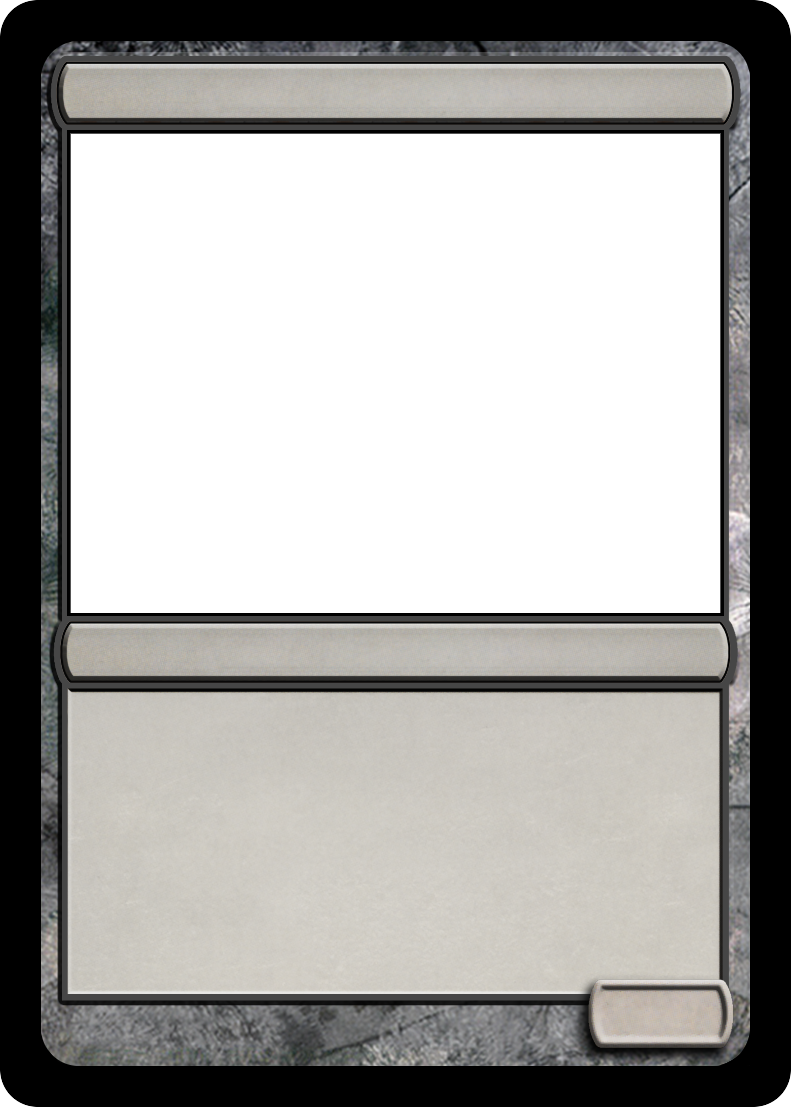
\includegraphics[width=\cardwidth cm, height=\cardheight cm]{fonds/fond_neutre.png}};

    %Titre
	\node[anchor=center] at (\titleX,\titleY) {\titlefont Mois de préavis};

	%Image
	\node[anchor=center] at (\imageX,\imageY) {
\includegraphics[width=\imageWidth px, height=\imageHeight px]{images/UO_45_preavis.jpg}};
	\node[anchor=center] at (6.1,4.5) {
\includegraphics[width=12 px, height=6 px]{fonds2/legacy.jpg}};

	%Type
	\node[anchor=center] at (\typeX,\typeY) {\typefont Neutre};

	%Description
	\node[anchor=north west, text width=5.6cm] (description) at (\descriptionX,\descriptionY) {\descriptionfont\setsize{6}Si la carte ANSSI est en jeu, vous pouvez immédiatement la faire pivoter d'un quart de tour, dans le sens que vous voulez. \par};

	%Numéro !!!!!PAS TOUCHE!!!!!
	\node[anchor=center] at (\numberX,\numberY) {\numberfont \cardnumber};
\end{tikzpicture}\verso %Verso


%%%%%%%%%%%%%%%%%%%%%%%%%%%%%%%%%%%%%%%%%%%%%%%%%
\begin{tikzpicture} %Recto
	%Fond
    \node[anchor=south west,inner sep=0] (carte) at (0,0) {
\includegraphics[width=7.1 cm, height=9.6 cm]{fonds/noir.png}};
    \node[anchor=center] at (carte.center) {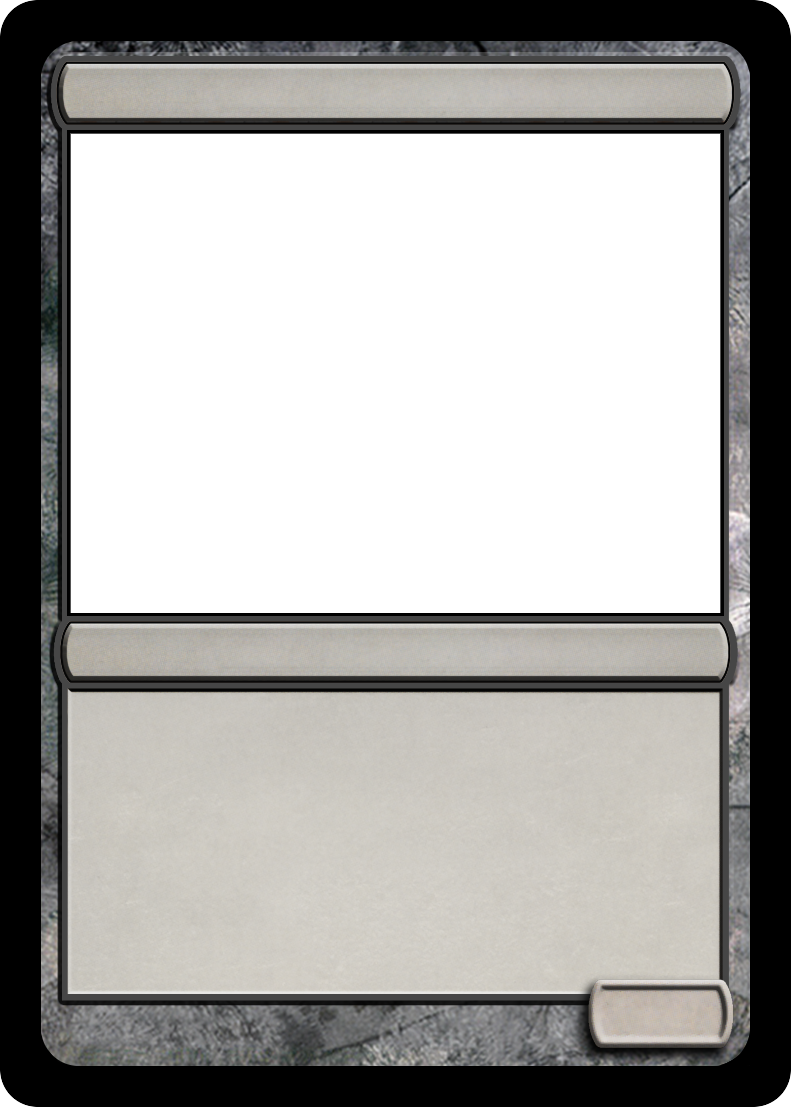
\includegraphics[width=\cardwidth cm, height=\cardheight cm]{fonds/fond_neutre.png}};

    %Titre
	\node[anchor=center] at (\titleX,\titleY) {\titlefont Note de frais Concur};

	%Image
	\node[anchor=center] at (\imageX,\imageY) {
\includegraphics[width=\imageWidth px, height=\imageHeight px]{images/UO_46_Concur.jpg}};
	\node[anchor=center] at (6.1,4.5) {
\includegraphics[width=12 px, height=6 px]{fonds2/legacy.jpg}};

	%Type
	\node[anchor=center] at (\typeX,\typeY) {\typefont Neutre};

	%Description
	\node[anchor=north west, text width=5.6cm] (description) at (\descriptionX,\descriptionY) {\descriptionfont\setsize{7}Un joueur choisi aléatoirement doit faire sa note de frais concur : il faut sommer toutes les valeurs des cartes dans le tas. Le manager et PMO peuvent vérifier. En cas d’erreur détecté par l’un deux, le joueur pioche 4 cartes.\par};

	%Punchline
	\node[anchor=north west, text width=5.6cm, below = 1pt of description] (punchline) {\punchlinefont\setsize{8}``N'oubliez pas de scanner le code barre avec les justificatifs.'\par};
	
	%Numéro !!!!!PAS TOUCHE!!!!!
	\node[anchor=center] at (\numberX,\numberY) {\numberfont \cardnumber};
\end{tikzpicture}\verso %Verso

\begin{tikzpicture} %Recto
	%Fond
    \node[anchor=south west,inner sep=0] (carte) at (0,0) {
\includegraphics[width=7.1 cm, height=9.6 cm]{fonds/noir.png}};
    \node[anchor=center] at (carte.center) {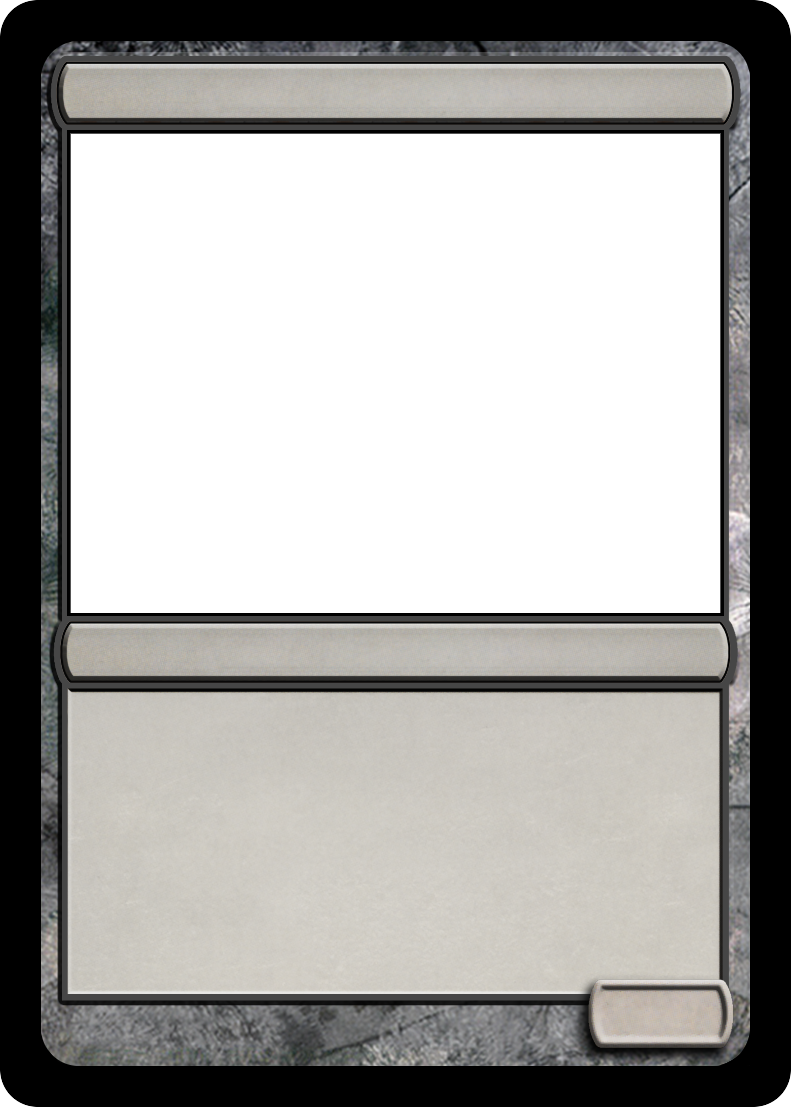
\includegraphics[width=\cardwidth cm, height=\cardheight cm]{fonds/fond_neutre.png}};

    %Titre
	\node[anchor=center] at (\titleX,\titleY) {\titlefont Cohue chez Elior};

	%Image
	\node[anchor=center] at (\imageX,\imageY) {
\includegraphics[width=\imageWidth px, height=\imageHeight px]{images/UO_60_Elior.jpg}};
	\node[anchor=center] at (6.1,4.5) {
\includegraphics[width=12 px, height=6 px]{fonds2/legacy.jpg}};

	%Type
	\node[anchor=center] at (\typeX,\typeY) {\typefont Neutre};

	%Description
	\node[anchor=north west, text width=5.6cm] (description) at (\descriptionX,\descriptionY) {\descriptionfont\setsize{7}Vite, Aurèle Dupont vous  entraîne à la cantine. Posez cette carte au centre de la table, suivi des autres joueurs. Le premier joueur qui pose sa carte au-dessus est le seul avec vous à ne pas piocher. Défaussez les cartes posées. Le dernier mange tout seul.\par};

	%Punchline
	\node[anchor=north west, text width=5.6cm, below = 1pt of description] (punchline) {\punchlinefont\setsize{7}``Il est 11h31, il faudrait voir à pas se foutre de ma gueule : j'ai faim.'\par};
	%Separateur !!!!!PAS TOUCHE!!!!!
	\fill[black,path fading=west] (description.south west) rectangle (punchline.north);
	\fill[black,path fading=east] (punchline.north) rectangle (description.south east);


	%Numéro !!!!!PAS TOUCHE!!!!!
	\node[anchor=center] at (\numberX,\numberY) {\numberfont \cardnumber};
\end{tikzpicture}\verso %Verso


\begin{tikzpicture} %Recto
	%Fond
    \node[anchor=south west,inner sep=0] (carte) at (0,0) {
\includegraphics[width=7.1 cm, height=9.6 cm]{fonds/noir.png}};
    \node[anchor=center] at (carte.center) {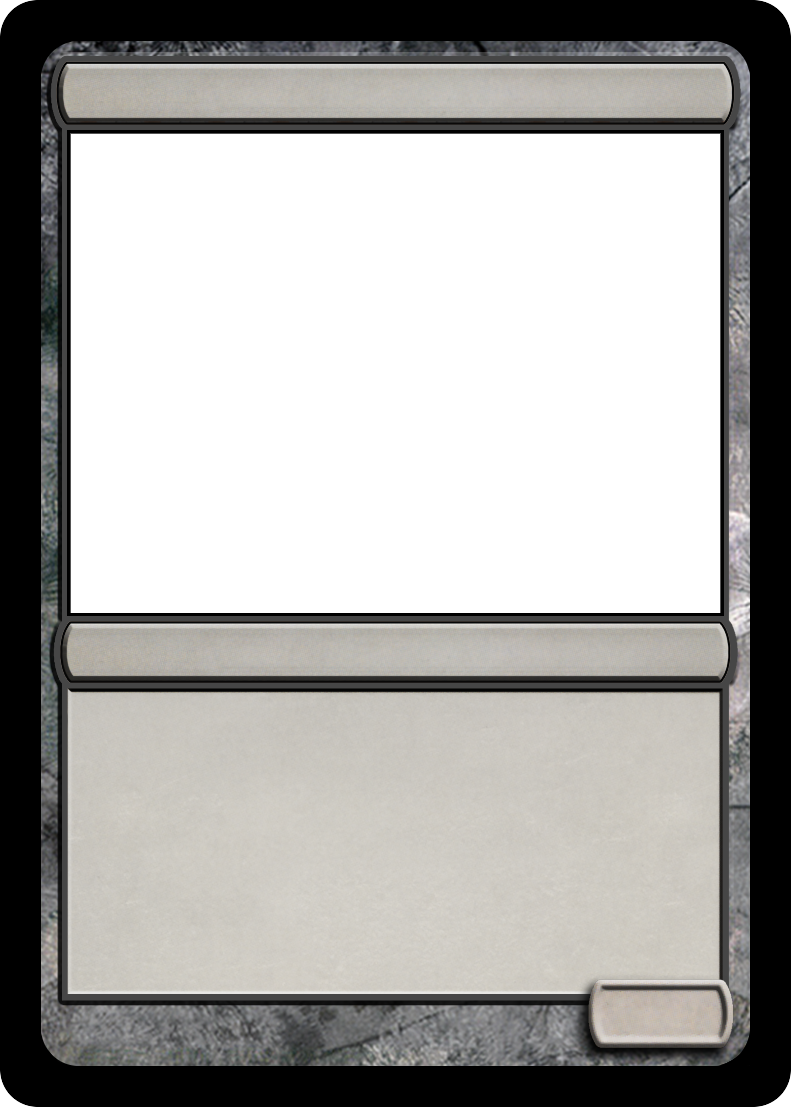
\includegraphics[width=\cardwidth cm, height=\cardheight cm]{fonds/fond_neutre.png}};

    %Titre
	\node[anchor=center] at (\titleX,\titleY) {\titlefont Reprise de code};

	%Image
	\node[anchor=center] at (\imageX,\imageY) {\includegraphics[width=\imageWidth px, height=\imageHeight px]{images/UO_62_code.jpg}};
	\node[anchor=center] at (6.1,4.5) {\includegraphics[width=12 px, height=6 px]{fonds2/legacy.jpg}};

	%Type
	\node[anchor=center] at (\typeX,\typeY) {\typefont Neutre};

	%Description
	\node[anchor=north west, text width=5.6cm] (description) at (\descriptionX,\descriptionY) {\descriptionfont\setsize{8} Vous devez reprendre le code d'un membre disparu du labo. Vous piochez une carte à tenter de faire fonctionner puis vous le refilez (cette carte) à un joueur de votre choix.\par};
	%Punchline
	\node[anchor=north west, text width=5.6cm, below = 1pt of description] (punchline) {\punchlinefont\setsize{8}``Quel cochon a codé if((test=failed)!=KO) return OK; ?!'\par};
	%Separateur !!!!!PAS TOUCHE!!!!!
	\fill[black,path fading=west] (description.south west) rectangle (punchline.north);
	\fill[black,path fading=east] (punchline.north) rectangle (description.south east);

	%Numéro !!!!!PAS TOUCHE!!!!!
	\node[anchor=center] at (\numberX,\numberY) {\numberfont \cardnumber};
\end{tikzpicture}\verso %Verso



\begin{tikzpicture} %Recto
	%Fond
    \node[anchor=south west,inner sep=0] (carte) at (0,0) {\includegraphics[width=7.1 cm, height=9.6 cm]{fonds/noir.png}};
    \node[anchor=center] at (carte.center) {\includegraphics[width=\cardwidth cm, height=\cardheight cm]{fonds/fond_neutre.png}};

    %Titre
	\node[anchor=center] at (\titleX,\titleY) {\titlefont Intervention Divine};

	%Image
	\node[anchor=center] at (\imageX,\imageY) {\includegraphics[width=\imageWidth px, height=\imageHeight px]{images/UO_62_intervention.jpg}};
	\node[anchor=center] at (6.1,4.5) {\includegraphics[width=12 px, height=6 px]{fonds2/legacy.jpg}};

	%Type
	\node[anchor=center] at (\typeX,\typeY) {\typefont Neutre};

	%Description
	\node[anchor=north west, text width=5.6cm] (description) at (\descriptionX,\descriptionY) {\descriptionfont\setsize{6} Votre directrice Odile Deraie vous interdit d'assister à une conférence à l'étranger. Jusqu'à la fin du tour, aucun joueur ne peut jouer de carte avec le titre conférence.\par};
	
	%Punchline
	\node[anchor=north west, text width=5.6cm, below = 1pt of description] (punchline) {\punchlinefont\setsize{8}``Deraie ! Odile Deraie !'\par};

	%Separateur !!!!!PAS TOUCHE!!!!!
	\fill[black,path fading=west] (description.south west) rectangle (punchline.north);
	\fill[black,path fading=east] (punchline.north) rectangle (description.south east);

	%Numéro !!!!!PAS TOUCHE!!!!!
	\node[anchor=center] at (\numberX,\numberY) {\numberfont \cardnumber};
\end{tikzpicture}\verso %Verso



\begin{tikzpicture} %Recto
	%Fond
    \node[anchor=south west,inner sep=0] (carte) at (0,0) {\includegraphics[width=7.1 cm, height=9.6 cm]{fonds/noir.png}};
    \node[anchor=center] at (carte.center) {\includegraphics[width=\cardwidth cm, height=\cardheight cm]{fonds/fond_neutre.png}};

    %Titre
	\node[anchor=center] at (\titleX,\titleY) {\titlefont Espion(ne) Russe};

	%Image
	\node[anchor=center] at (\imageX,\imageY) {\includegraphics[width=\imageWidth px, height=\imageHeight px]{images/UO_63_espion.jpg}};
	\node[anchor=center] at (6.1,4.5) {\includegraphics[width=12 px, height=6 px]{fonds2/legacy.jpg}};

	%Type
	\node[anchor=center] at (\typeX,\typeY) {\typefont Neutre};

	%Description
	\node[anchor=north west, text width=5.6cm] (description) at (\descriptionX,\descriptionY) {\descriptionfont\setsize{8} Jouez cette carte uniquement si vous êtes habilité. Natashatte vous donne la possibilité de défausser deux cartes en échange de votre habilitation.\par};
	
	%Punchline
	\node[anchor=north west, text width=5.6cm, below = 1pt of description] (punchline) {\punchlinefont\setsize{8} Je trrouver vous très beau.\par};
	%Separateur !!!!!PAS TOUCHE!!!!!
	\fill[black,path fading=west] (description.south west) rectangle (punchline.north);
	\fill[black,path fading=east] (punchline.north) rectangle (description.south east);

	
	%Numéro !!!!!PAS TOUCHE!!!!!
	\node[anchor=center] at (\numberX,\numberY) {\numberfont \cardnumber};
\end{tikzpicture}\verso %Verso

\begin{tikzpicture} %Recto
	%Fond
    \node[anchor=south west,inner sep=0] (carte) at (0,0) {\includegraphics[width=7.1 cm, height=9.6 cm]{fonds/noir.png}};
    \node[anchor=center] at (carte.center) {\includegraphics[width=\cardwidth cm, height=\cardheight cm]{fonds/fond_neutre.png}};

    %Titre
	\node[anchor=center] at (\titleX,\titleY) {\titlefont DPA};

	%Image
	\node[anchor=center] at (\imageX,\imageY) {\includegraphics[width=\imageWidth px, height=\imageHeight px]{images/DPA.jpg}};
	\node[anchor=center] at (6.1,4.5) {\includegraphics[width=12 px, height=6 px]{fonds2/legacy.jpg}};

	%Type
	\node[anchor=center] at (\typeX,\typeY) {\typefont Neutre};

	%Description
	\node[anchor=north west, text width=5.6cm] (description) at (\descriptionX,\descriptionY) {\descriptionfont\setsize{7} Vous êtes un expert DPA. Demandez à un joueur de montrer le bord de ses cartes. Vous pouvez en jouer une de votre choix immédiatement et appliquer son effet. Le joueur attaqué pioche une carte.\par};

	\node[anchor=north west, text width=5.6cm, below = 1pt of description] (punchline) {\punchlinefont\setsize{7}``Une contremesure serait que toutes les cartes soient blanches. Mais ce serait moche.		''\par};

	%Separateur !!!!!PAS TOUCHE!!!!!
	\fill[black,path fading=west] (description.south west) rectangle (punchline.north);
	\fill[black,path fading=east] (punchline.north) rectangle (description.south east);

	%Numéro !!!!!PAS TOUCHE!!!!!
	\node[anchor=center] at (\numberX,\numberY) {\numberfont \cardnumber};
\end{tikzpicture}\verso %Verso

\begin{tikzpicture} %Recto
	%Fond
    \node[anchor=south west,inner sep=0] (carte) at (0,0) {\includegraphics[width=7.1 cm, height=9.6 cm]{fonds/noir.png}};
    \node[anchor=center] at (carte.center) {\includegraphics[width=\cardwidth cm, height=\cardheight cm]{fonds/fond_neutre.png}};

    %Titre
	\node[anchor=center] at (\titleX,\titleY) {\titlefont Zumba};

	%Image
	\node[anchor=center] at (\imageX,\imageY) {\includegraphics[width=\imageWidth px, height=\imageHeight px]{images/UO_65_Zumba.jpg}};
	\node[anchor=center] at (6.1,4.5) {\includegraphics[width=12 px, height=6 px]{fonds2/legacy.jpg}};

	%Type
	\node[anchor=center] at (\typeX,\typeY) {\typefont Neutre};

	%Description
	\node[anchor=north west, text width=5.6cm] (description) at (\descriptionX,\descriptionY) {\descriptionfont\setsize{8} Plutôt que de travailler ou de faire du sport, vous décidez d'aller à la Zumba.\par};
	
	\node[anchor=north west, text width=5.6cm, below = 1pt of description] (punchline) {\punchlinefont\setsize{8}``Tout comme la Zumba, cette carte ne sert à rien.''\par};

	%Separateur !!!!!PAS TOUCHE!!!!!
	\fill[black,path fading=west] (description.south west) rectangle (punchline.north);
	\fill[black,path fading=east] (punchline.north) rectangle (description.south east);

	%Numéro !!!!!PAS TOUCHE!!!!!
	\node[anchor=center] at (\numberX,\numberY) {\numberfont \cardnumber};
\end{tikzpicture}\verso %Verso



\begin{tikzpicture} %Recto
	%Fond
    \node[anchor=south west,inner sep=0] (carte) at (0,0) {\includegraphics[width=7.1 cm, height=9.6 cm]{fonds/noir.png}};
    \node[anchor=center] at (carte.center) {\includegraphics[width=\cardwidth cm, height=\cardheight cm]{fonds/fond_neutre.png}};

    %Titre
	\node[anchor=center] at (\titleX,\titleY) {\titlefont Météo};

	%Image
	\node[anchor=center] at (\imageX,\imageY) {\includegraphics[width=\imageWidth px, height=\imageHeight px]{images/UO_67_Meteo.jpg}};
	\node[anchor=center] at (6.1,4.5) {\includegraphics[width=12 px, height=6 px]{fonds2/legacy.jpg}};

	%Type
	\node[anchor=center] at (\typeX,\typeY) {\typefont Neutre};

	%Description
	\node[anchor=north west, text width=5.6cm] (description) at (\descriptionX,\descriptionY) {\descriptionfont\setsize{8} Chaque joueur doit donner la température qu'il fait à Marseille. Le plus proche défausse une carte.\par};
	
	%Punchline
	\node[anchor=north west, text width=5.6cm, below = 1pt of description] (punchline) {\punchlinefont\setsize{8}``Si, il fait très beau. \`A Marseille''\par};

	%Separateur !!!!!PAS TOUCHE!!!!!
	\fill[black,path fading=west] (description.south west) rectangle (punchline.north);
	\fill[black,path fading=east] (punchline.north) rectangle (description.south east);

	%Numéro !!!!!PAS TOUCHE!!!!!
	\node[anchor=center] at (\numberX,\numberY) {\numberfont \cardnumber};
\end{tikzpicture}\verso %Verso



\begin{tikzpicture} %Recto
	%Fond
    \node[anchor=south west,inner sep=0] (carte) at (0,0) {\includegraphics[width=7.1 cm, height=9.6 cm]{fonds/noir.png}};
    \node[anchor=center] at (carte.center) {\includegraphics[width=\cardwidth cm, height=\cardheight cm]{fonds/fond_neutre.png}};

    %Titre
	\node[anchor=center] at (\titleX,\titleY) {\titlefont Spec. Incompréhensible};

	%Image
	\node[anchor=center] at (\imageX,\imageY) {\includegraphics[width=\imageWidth px, height=\imageHeight px]{images/UO_69_spec.jpg}};
	\node[anchor=center] at (6.1,4.5) {\includegraphics[width=12 px, height=6 px]{fonds2/legacy.jpg}};

	%Type
	\node[anchor=center] at (\typeX,\typeY) {\typefont Neutre};

	%Description
	\node[anchor=north west, text width=5.6cm] (description) at (\descriptionX,\descriptionY) {\descriptionfont\setsize{7} L’algorithme Jason/Morville est une vraie plaie. A croire que cette spécification a été écrite avec les pieds. Regardez le premier mot de la dernière carte du tas et écrivez-le avec un stylo entre les pieds. Si un joueur réussit à décoder cette bouse, il aura bien mérité de défausser une carte et vous aussi !!!!\par};
	

	%Numéro !!!!!PAS TOUCHE!!!!!
	\node[anchor=center] at (\numberX,\numberY) {\numberfont \cardnumber};
\end{tikzpicture}\verso %Verso


\begin{tikzpicture} %Recto
	%Fond
    \node[anchor=south west,inner sep=0] (carte) at (0,0) {\includegraphics[width=7.1 cm, height=9.6 cm]{fonds/noir.png}};
    \node[anchor=center] at (carte.center) {\includegraphics[width=\cardwidth cm, height=\cardheight cm]{fonds/fond_neutre.png}};

    %Titre
	\node[anchor=center] at (\titleX,\titleY) {\titlefont On en a gros !};

	%Image
	\node[anchor=center] at (\imageX,\imageY) {\includegraphics[width=\imageWidth px, height=\imageHeight px]{images/UO_68_gros.jpg}};
	\node[anchor=center] at (6.1,4.5) {\includegraphics[width=12 px, height=6 px]{fonds2/legacy.jpg}};

	%Type
	\node[anchor=center] at (\typeX,\typeY) {\typefont Neutre};

	%Description
	\node[anchor=north west, text width=5.6cm] (description) at (\descriptionX,\descriptionY) {\descriptionfont\setsize{7} Les syndicats appellent au débrayage. Révélez chacun une carte du tas, le joueur qui en a le plus gros (obtenant la valeur maximale) défausse une carte. Jetez tous ce foutoir pioché avec les scandaleuses propositions de la direction.\par};
	
	%Punchline
	\node[anchor=north west, text width=5.6cm, below = 1pt of description] (punchline) {\punchlinefont\setsize{8}``On veut être traités en tant que tel !''\par};

	%Separateur !!!!!PAS TOUCHE!!!!!
	\fill[black,path fading=west] (description.south west) rectangle (punchline.north);
	\fill[black,path fading=east] (punchline.north) rectangle (description.south east);

	%Numéro !!!!!PAS TOUCHE!!!!!
	\node[anchor=center] at (\numberX,\numberY) {\numberfont \cardnumber};
\end{tikzpicture}\verso %Verso



\begin{tikzpicture} %Recto
	%Fond
    \node[anchor=south west,inner sep=0] (carte) at (0,0) {\includegraphics[width=7.1 cm, height=9.6 cm]{fonds/noir.png}};
    \node[anchor=center] at (carte.center) {\includegraphics[width=\cardwidth cm, height=\cardheight cm]{fonds/fond_neutre.png}};

    %Titre
	\node[anchor=center] at (\titleX,\titleY) {\titlefont Tournoi LCH de squash :};

	%Image
	\node[anchor=center] at (\imageX,\imageY) {\includegraphics[width=\imageWidth px, height=\imageHeight px]{images/UO_71_squash.jpg}};
	\node[anchor=center] at (6.1,4.5) {\includegraphics[width=12 px, height=6 px]{fonds2/legacy.jpg}};

	%Type
	\node[anchor=center] at (\typeX,\typeY) {\typefont Neutre};

	%Description
	\node[anchor=north west, text width=5.6cm] (description) at (\descriptionX,\descriptionY) {\descriptionfont\setsize{8}Jetez un objet en lobe au milieu de la table. Le joueur qui l’attrape défausse une carte. Si un joueur s'appelle David, écoutez le longuement expliquer comment il a gagné/perdu.\par};
	
	%Punchline
	\node[anchor=north west, text width=5.6cm, below = 1pt of description] (punchline) {\punchlinefont\setsize{8}``Le squash – Toujours le sport préféré des connards''\par};

	%Separateur !!!!!PAS TOUCHE!!!!!
	\fill[black,path fading=west] (description.south west) rectangle (punchline.north);
	\fill[black,path fading=east] (punchline.north) rectangle (description.south east);

	%Numéro !!!!!PAS TOUCHE!!!!!
	\node[anchor=center] at (\numberX,\numberY) {\numberfont \cardnumber};
\end{tikzpicture}\verso %Verso



\begin{tikzpicture} %Recto
	%Fond
    \node[anchor=south west,inner sep=0] (carte) at (0,0) {\includegraphics[width=7.1 cm, height=9.6 cm]{fonds/noir.png}};
    \node[anchor=center] at (carte.center) {\includegraphics[width=\cardwidth cm, height=\cardheight cm]{fonds/fond_neutre.png}};

    %Titre
	\node[anchor=center] at (\titleX,\titleY) {\titlefont Transfert CHOCE };

	%Image
	\node[anchor=center] at (\imageX,\imageY) {\includegraphics[width=\imageWidth px, height=\imageHeight px]{images/transfert_CHOCE.jpg}};
	\node[anchor=center] at (6.1,4.5) {\includegraphics[width=12 px, height=6 px]{fonds2/legacy.jpg}};

	%Type
	\node[anchor=center] at (\typeX,\typeY) {\typefont Neutre};

	%Description
	\node[anchor=north west, text width=5.6cm] (description) at (\descriptionX,\descriptionY) {\descriptionfont\setsize{6}Prétextant lâchement ne pas avoir de compte, choisissez un joueur qui se lève, prend une carte au hasard dans votre main l’acidifie en la frottant sur la station blanche (le tas) et l’échange avec la carte d’un troisième joueur. De toute façon CHOLET vous redemandera une mise à jour demain.\par};
	
	%Punchline
	\node[anchor=north west, text width=5.6cm, below = 1pt of description] (punchline) {\punchlinefont\setsize{8}``Si, si j'ai fait la demande.''\par};

	%Separateur !!!!!PAS TOUCHE!!!!!
	\fill[black,path fading=west] (description.south west) rectangle (punchline.north);
	\fill[black,path fading=east] (punchline.north) rectangle (description.south east);

	%Numéro !!!!!PAS TOUCHE!!!!!
	\node[anchor=center] at (\numberX,\numberY) {\numberfont \cardnumber};
\end{tikzpicture}\verso %Verso
	

\begin{tikzpicture} %Recto
	%Fond
    \node[anchor=south west,inner sep=0] (carte) at (0,0) {\includegraphics[width=7.1 cm, height=9.6 cm]{fonds/noir.png}};
    \node[anchor=center] at (carte.center) {\includegraphics[width=\cardwidth cm, height=\cardheight cm]{fonds/fond_neutre.png}};

    %Titre
	\node[anchor=center] at (\titleX,\titleY) {\titlefont Visite surprise de la DPSD !!!};

	%Image
	\node[anchor=center] at (\imageX,\imageY) {\includegraphics[width=\imageWidth px, height=\imageHeight px]{images/UO_73_DPSD.jpg}};
	\node[anchor=center] at (6.1,4.5) {\includegraphics[width=12 px, height=6 px]{fonds2/legacy.jpg}};

	%Type
	\node[anchor=center] at (\typeX,\typeY) {\typefont Neutre};

	%Description
	\node[anchor=north west, text width=5.6cm] (description) at (\descriptionX,\descriptionY) {\descriptionfont\setsize{7}Vite, vite! Planquez tous les documents secrets dans le coffre. Dans la précipitation, les 5 et le S de nato Secret ont été confondus ! Tous les joueurs peuvent défausser les cartes de valeur 5.\par};
	
	%Punchline
	\node[anchor=north west, text width=5.6cm, below = 1pt of description] (punchline) {\punchlinefont\setsize{8}``C'est un beau bordel, mais toujours moins que dans le tiroir de votre chef.''\par};

	%Separateur !!!!!PAS TOUCHE!!!!!
	\fill[black,path fading=west] (description.south west) rectangle (punchline.north);
	\fill[black,path fading=east] (punchline.north) rectangle (description.south east);

	%Numéro !!!!!PAS TOUCHE!!!!!
	\node[anchor=center] at (\numberX,\numberY) {\numberfont \cardnumber};
\end{tikzpicture}\verso %Verso


\begin{tikzpicture} %Recto
	%Fond
    \node[anchor=south west,inner sep=0] (carte) at (0,0) {\includegraphics[width=7.1 cm, height=9.6 cm]{fonds/noir.png}};
    \node[anchor=center] at (carte.center) {\includegraphics[width=\cardwidth cm, height=\cardheight cm]{fonds/fond_neutre.png}};

    %Titre
	\node[anchor=center] at (\titleX,\titleY) {\titlefont\setsize{7}Offre d’emploi sur la mailing list crypto\par};

	%Image
	\node[anchor=center] at (\imageX,\imageY) {\includegraphics[width=\imageWidth px, height=\imageHeight px]{images/offreanssi.jpg}};
	\node[anchor=center] at (6.1,4.5) {\includegraphics[width=12 px, height=6 px]{fonds2/legacy.jpg}};

	%Type
	\node[anchor=center] at (\typeX,\typeY) {\typefont Neutre};

	%Description
	\node[anchor=north west, text width=5.6cm] (description) at (\descriptionX,\descriptionY) {\descriptionfont\setsize{7}Le premier joueur qui pose sa main sur le tas défausse une carte. Sauf vous qui êtes occupé à lire bêtement ce texte et laissez filer une occasion de quitter cet asile de fous.\par};
	
	%Punchline
	\node[anchor=north west, text width=5.6cm, below = 1pt of description] (punchline) {\punchlinefont\setsize{8}``Salaire attractif, poste technique, carte Zone 1-2 uniquement.''\par};

	%Separateur !!!!!PAS TOUCHE!!!!!
	\fill[black,path fading=west] (description.south west) rectangle (punchline.north);
	\fill[black,path fading=east] (punchline.north) rectangle (description.south east);

	%Numéro !!!!!PAS TOUCHE!!!!!
	\node[anchor=center] at (\numberX,\numberY) {\numberfont \cardnumber};
\end{tikzpicture}\verso %Verso

%%%%%%%%%%%%%%%%%%%%%%%%%%%%%%%%%%%%%%%%%%

\begin{tikzpicture} %Recto
	%Fond
    \node[anchor=south west,inner sep=0] (carte) at (0,0) {\includegraphics[width=7.1 cm, height=9.6 cm]{fonds/noir.png}};
    \node[anchor=center] at (carte.center) {\includegraphics[width=\cardwidth cm, height=\cardheight cm]{fonds/fond_neutre.png}};

    %Titre
	\node[anchor=center] at (\titleX,\titleY) {\titlefont Rho de pollard };

	%Image
	\node[anchor=center] at (\imageX,\imageY) {\includegraphics[width=\imageWidth px, height=\imageHeight px]{images/rho_pollard.jpg}};
	\node[anchor=center] at (6.1,4.5) {\includegraphics[width=12 px, height=6 px]{fonds2/legacy.jpg}};

	%Type
	\node[anchor=center] at (\typeX,\typeY) {\typefont Neutre};

	%Description
	\node[anchor=north west, text width=5.6cm] (description) at (\descriptionX,\descriptionY) {\descriptionfont\setsize{6}Vous aidez le LORIA à battre son record de cryptanalyse. Debout sur votre chaise, piochez puis lâchez une carte qui doit virevolter le plus possible sur elle-même. Si elle tombe sans bug (recto visible) et que sa valeur collisionne avec une carte du tas, vous avez trouvé une collision et cassé le log discret ! Défaussez alors une carte, sinon piochez.\par };

	%Punchline
	\node[anchor=north west, text width=5.6cm, below = 1pt of description] (punchline) {\punchlinefont\setsize{6}``Pensez à la planète avant de lancer ces calculs inutiles sur le server.\par''};

	%Separateur !!!!!PAS TOUCHE!!!!!
	\fill[black,path fading=west] (description.south west) rectangle (punchline.north);
	\fill[black,path fading=east] (punchline.north) rectangle (description.south east);
	%Numéro !!!!!PAS TOUCHE!!!!!
	\node[anchor=center] at (\numberX,\numberY) {\numberfont \cardnumber};
\end{tikzpicture}\verso %Verso
 
%%%%%%%%%%%%%%%%%%%%%%%%%%%%%%%%%%%%%%%%%%

\begin{tikzpicture} %Recto
	%Fond
    \node[anchor=south west,inner sep=0] (carte) at (0,0) {\includegraphics[width=7.1 cm, height=9.6 cm]{fonds/noir.png}};
    \node[anchor=center] at (carte.center) {\includegraphics[width=\cardwidth cm, height=\cardheight cm]{fonds/fond_neutre.png}};

    %Titre
	\node[anchor=center] at (\titleX,\titleY) {\titlefont Sens des données  };

	%Image
	\node[anchor=center] at (\imageX,\imageY) {\includegraphics[width=\imageWidth px, height=\imageHeight px]{images/Sens_des_données.jpg}};
	\node[anchor=center] at (6.1,4.5) {\includegraphics[width=12 px, height=6 px]{fonds2/legacy.jpg}};

	%Type
	\node[anchor=center] at (\typeX,\typeY) {\typefont Neutre};

	%Description
	\node[anchor=north west, text width=5.6cm] (description) at (\descriptionX,\descriptionY) {\descriptionfont\setsize{7}V: @zjfna !! Encore un problème de MSB, LSB, ByteString, Endianess. Révélez secrètement une carte du tas. Epelez le mot de la carte le plus long à l’envers. Le premier joueur qui devine juste défausse une carte. Chaque erreur d’un joueur lui fait piocher une carte.\par};
	
	%Punchline
	\node[anchor=north west, text width=5.6cm, below = 1pt of description] (punchline) {\punchlinefont\setsize{8}``erocne! tuz !''\par};

	%Separateur !!!!!PAS TOUCHE!!!!!
	\fill[black,path fading=west] (description.south west) rectangle (punchline.north);
	\fill[black,path fading=east] (punchline.north) rectangle (description.south east);

	%Numéro !!!!!PAS TOUCHE!!!!!
	\node[anchor=center] at (\numberX,\numberY) {\numberfont \cardnumber};
\end{tikzpicture}\verso %Verso

%%%%%%%%%%%%%%%%%%%%%%%%%%%%%%%%%%%%%%%%%%

\begin{tikzpicture} %Recto
	%Fond
    \node[anchor=south west,inner sep=0] (carte) at (0,0) {\includegraphics[width=7.1 cm, height=9.6 cm]{fonds/noir.png}};
    \node[anchor=center] at (carte.center) {\includegraphics[width=\cardwidth cm, height=\cardheight cm]{fonds/fond_neutre.png}};

    %Titre
	\node[anchor=center] at (\titleX,\titleY) {\titlefont Arnaque à la blockchain };

	%Image
	\node[anchor=center] at (\imageX,\imageY) {\includegraphics[width=\imageWidth px, height=\imageHeight px]{images/UO_74_Blockchain.jpg}};
	\node[anchor=center] at (6.1,4.5) {\includegraphics[width=12 px, height=6 px]{fonds2/legacy.jpg}};

	%Type
	\node[anchor=center] at (\typeX,\typeY) {\typefont Neutre};

	%Description
	\node[anchor=north west, text width=5.6cm] (description) at (\descriptionX,\descriptionY) {\descriptionfont\setsize{6}Ah ah ah sacrés cryptologues ! Ils ont réussi à refourguer la création d’une blockchain, maintenant ils doivent faire tourner une proof of work qui va ruiner le climat. Chaque joueur pioche une carte puis vous posez une carte de votre choix. Chacun à son tour un joueur peut poser une carte de valeur supérieure avant que l’escroquerie et la bulle n'explosent.\par};
	
	%Punchline
	\node[anchor=north west, text width=5.6cm, below = 1pt of description] (punchline) {\punchlinefont\setsize{8}``La chasse au pigeon est ouverte !''\par};

	%Separateur !!!!!PAS TOUCHE!!!!!
	\fill[black,path fading=west] (description.south west) rectangle (punchline.north);
	\fill[black,path fading=east] (punchline.north) rectangle (description.south east);

	%Numéro !!!!!PAS TOUCHE!!!!!
	\node[anchor=center] at (\numberX,\numberY) {\numberfont \cardnumber};
\end{tikzpicture}\verso %Verso


\begin{tikzpicture} %Recto
	%Fond
    \node[anchor=south west,inner sep=0] (carte) at (0,0) {\includegraphics[width=7.1 cm, height=9.6 cm]{fonds/noir.png}};
    \node[anchor=center] at (carte.center) {\includegraphics[width=\cardwidth cm, height=\cardheight cm]{fonds/fond_neutre.png}};

    %Titre
	\node[anchor=center] at (\titleX,\titleY) {\titlefont Calcul de CRC };

	%Image
	\node[anchor=center] at (\imageX,\imageY) {\includegraphics[width=\imageWidth px, height=\imageHeight px]{images/CRC.png}};
	\node[anchor=center] at (6.1,4.5) {\includegraphics[width=12 px, height=6 px]{fonds2/legacy.jpg}};

	%Type
	\node[anchor=center] at (\typeX,\typeY) {\typefont Neutre};

	%Description
	\node[anchor=north west, text width=5.6cm] (description) at (\descriptionX,\descriptionY) {\descriptionfont\setsize{8}Révélez 4 cartes du tas. Tous les joueurs dont au moins une carte vaut 1 plus la somme de ces cartes modulo 8 peut défausser cette carte (une seule).\par};
	

	%Numéro !!!!!PAS TOUCHE!!!!!
	\node[anchor=center] at (\numberX,\numberY) {\numberfont \cardnumber};
 
\end{tikzpicture}\verso %Verso


\begin{tikzpicture} %Recto
	%Fond
    \node[anchor=south west,inner sep=0] (carte) at (0,0) {\includegraphics[width=7.1 cm, height=9.6 cm]{fonds/noir.png}};
    \node[anchor=center] at (carte.center) {\includegraphics[width=\cardwidth cm, height=\cardheight cm]{fonds/fond_neutre.png}};

    %Titre
	\node[anchor=center] at (\titleX,\titleY) {\titlefont Saisie de mot de passe };

	%Image
	\node[anchor=center] at (\imageX,\imageY) {\includegraphics[width=\imageWidth px, height=\imageHeight px]{images/motdepasse.jpg}};
	\node[anchor=center] at (6.1,4.5) {\includegraphics[width=12 px, height=6 px]{fonds2/legacy.jpg}};

	%Type
	\node[anchor=center] at (\typeX,\typeY) {\typefont Neutre};

	%Description
	\node[anchor=north west, text width=5.6cm] (description) at (\descriptionX,\descriptionY) {\descriptionfont\setsize{6}Vous avez tous noté votre mot de passe sur la valeur de carte jouée le tour précédent. Sans regarder le tas, chacun doit dire la valeur correcte sous peine d’appeler DSI. Si entre-temps le tas a été remélangé, pas de chance ! Vous étiez tous en vacances pendant le renouvellement, appelez. Tous les joueurs qui appellent Satan doivent dire 3915 et piocher une carte.\par};
	
	%Punchline
	\node[anchor=north west, text width=5.6cm, below = 1pt of description] (punchline) {\punchlinefont\setsize{8}``Rhaa, totocaca ou algoalgo, je sais plus.''\par};

	%Separateur !!!!!PAS TOUCHE!!!!!
	\fill[black,path fading=west] (description.south west) rectangle (punchline.north);
	\fill[black,path fading=east] (punchline.north) rectangle (description.south east);


	%Numéro !!!!!PAS TOUCHE!!!!!
	\node[anchor=center] at (\numberX,\numberY) {\numberfont \cardnumber};
 
\end{tikzpicture}\verso %Verso


\begin{tikzpicture} %Recto
	%Fond
    \node[anchor=south west,inner sep=0] (carte) at (0,0) {\includegraphics[width=7.1 cm, height=9.6 cm]{fonds/noir.png}};
    \node[anchor=center] at (carte.center) {\includegraphics[width=\cardwidth cm, height=\cardheight cm]{fonds/fond_malus.png}};

    %Titre
	\node[anchor=center] at (\titleX,\titleY) {\titlefont Collègue cafteur };

	%Image
	\node[anchor=center] at (\imageX,\imageY) {\includegraphics[width=\imageWidth px, height=\imageHeight px]{images/UO_83_cafteur.jpg}};
	\node[anchor=center] at (6.1,4.5) {\includegraphics[width=12 px, height=6 px]{fonds2/legacy.jpg}};

	%Type
	\node[anchor=center] at (\typeX,\typeY) {\typefont Malus (Interruption)};

	%Description
	\node[anchor=north west, text width=5.6cm] (description) at (\descriptionX,\descriptionY) {\descriptionfont\setsize{6}Votre collègue cafteur est à l’affut du moindre faux pas d’un de ses collègues pour tout cafter au manager. Vous ne pouvez pas défausser cette carte. Par contre dès qu’un joueur commet une erreur de jeux, de calcul, de français, caftez-le immédiatement au manager en jouant cette carte. Le joueur dénoncé pioche une carte.\par};
	
	%Punchline
	\node[anchor=north west, text width=5.6cm, below = 1pt of description] (punchline) {\punchlinefont\setsize{8}``Nadia Hémorroïd est toujours vigilante.''\par};

	%Separateur !!!!!PAS TOUCHE!!!!!
	\fill[black,path fading=west] (description.south west) rectangle (punchline.north);
	\fill[black,path fading=east] (punchline.north) rectangle (description.south east);


	%Numéro !!!!!PAS TOUCHE!!!!!
	\node[anchor=center] at (\numberX,\numberY) {\numberfont \cardnumber};
 
\end{tikzpicture}\verso %Verso


\begin{tikzpicture} %Recto
	%Fond
    \node[anchor=south west,inner sep=0] (carte) at (0,0) {\includegraphics[width=7.1 cm, height=9.6 cm]{fonds/noir.png}};
    \node[anchor=center] at (carte.center) {\includegraphics[width=\cardwidth cm, height=\cardheight cm]{fonds/fond_neutre.png}};

    %Titre
	\node[anchor=center] at (\titleX,\titleY) {\titlefont Peu scrupuleux};

	%Image
	\node[anchor=center] at (\imageX,\imageY) {\includegraphics[width=\imageWidth px, height=\imageHeight px]{images/UO_84_peuscrup.jpg}};
	\node[anchor=center] at (6.1,4.5) {\includegraphics[width=12 px, height=6 px]{fonds2/legacy.jpg}};

	%Type
	\node[anchor=center] at (\typeX,\typeY) {\typefont Neutre};

	%Description
	\node[anchor=north west, text width=5.6cm] (description) at (\descriptionX,\descriptionY) {\descriptionfont\setsize{6} Vous ne pouvez pas défausser cette carte. Si le manager est absent (pas choisi ce tour de jeux) vous pouvez la jouer, puis quitter la table jusqu’au prochain tour de jeux. Vous n’êtes concernés par aucune action/carte/bonus/malus ou surcharge de vos imbéciles de collègues fayots.\par};

	%Punchline
	\node[anchor=north west, text width=5.6cm, below = 1pt of description] (punchline) {\punchlinefont\setsize{8}``Vivement le prochain barbecue.''\par};

	%Separateur !!!!!PAS TOUCHE!!!!!
	\fill[black,path fading=west] (description.south west) rectangle (punchline.north);
	\fill[black,path fading=east] (punchline.north) rectangle (description.south east);

	%Numéro !!!!!PAS TOUCHE!!!!!
	\node[anchor=center] at (\numberX,\numberY) {\numberfont \cardnumber};
 
\end{tikzpicture}\verso %Verso



\begin{tikzpicture} %Recto
	%Fond
    \node[anchor=south west,inner sep=0] (carte) at (0,0) {\includegraphics[width=7.1 cm, height=9.6 cm]{fonds/noir.png}};
    \node[anchor=center] at (carte.center) {\includegraphics[width=\cardwidth cm, height=\cardheight cm]{fonds/fond_neutre.png}};

    %Titre
	\node[anchor=center] at (\titleX,\titleY) {\titlefont Show Log SVN};

	%Image
	\node[anchor=center] at (\imageX,\imageY) {\includegraphics[width=\imageWidth px, height=\imageHeight px]{images/UO_85_SVN.jpg}};
	\node[anchor=center] at (6.1,4.5) {\includegraphics[width=12 px, height=6 px]{fonds2/legacy.jpg}};

	%Type
	\node[anchor=center] at (\typeX,\typeY) {\typefont Neutre};

	%Description
	\node[anchor=north west, text width=5.6cm] (description) at (\descriptionX,\descriptionY) {\descriptionfont\setsize{8}Vous inspectez minutieusement le SVN à la recherche d’une version livrée il y a 6 ans. Tirez aléatoirement une valeur. Rejouez une carte du tas de votre choix avec la même valeur. En cas d’absence, vous devez tout recoder et piochez une carte.\par};

	%Numéro !!!!!PAS TOUCHE!!!!!
	\node[anchor=center] at (\numberX,\numberY) {\numberfont \cardnumber};
 
\end{tikzpicture}\verso %Verso



\begin{tikzpicture} %Recto
	%Fond
    \node[anchor=south west,inner sep=0] (carte) at (0,0) {\includegraphics[width=7.1 cm, height=9.6 cm]{fonds/noir.png}};
    \node[anchor=center] at (carte.center) {\includegraphics[width=\cardwidth cm, height=\cardheight cm]{fonds/fond_neutre.png}};

    %Titre
	\node[anchor=center] at (\titleX,\titleY) {\titlefont Période des EAA};

	%Image
	\node[anchor=center] at (\imageX,\imageY) {\includegraphics[width=\imageWidth px, height=\imageHeight px]{images/UO_86_EAA.jpg}};
	\node[anchor=center] at (6.1,4.5) {\includegraphics[width=12 px, height=6 px]{fonds2/legacy.jpg}};

	%Type
	\node[anchor=center] at (\typeX,\typeY) {\typefont Neutre};

	%Description
	\node[anchor=north west, text width=5.6cm] (description) at (\descriptionX,\descriptionY) {\descriptionfont\setsize{8}Chaque joueur révèle une carte pour connaître son niveau de performance cette année.\\1 : Inadéquation, piochez deux cartes,\\2-3 : En construction, piochez une carte.\\4-5 : Adéquation.\\6-7 : Maîtrise : défaussez une carte.\\8 : Excellence : défaussez deux cartes.\par};

	%Numéro !!!!!PAS TOUCHE!!!!!
	\node[anchor=center] at (\numberX,\numberY) {\numberfont \cardnumber};
 
\end{tikzpicture}\verso %Verso




\begin{tikzpicture} %Recto
	%Fond
    \node[anchor=south west,inner sep=0] (carte) at (0,0) {\includegraphics[width=7.1 cm, height=9.6 cm]{fonds/noir.png}};
    \node[anchor=center] at (carte.center) {\includegraphics[width=\cardwidth cm, height=\cardheight cm]{fonds/fond_neutre.png}};

    %Titre
	\node[anchor=center] at (\titleX,\titleY) {\titlefont Relecture de brevet};

	%Image
	\node[anchor=center] at (\imageX,\imageY) {\includegraphics[width=\imageWidth px, height=\imageHeight px]{images/Relecture.jpg}};
	\node[anchor=center] at (6.1,4.5) {\includegraphics[width=12 px, height=6 px]{fonds2/legacy.jpg}};

	%Type
	\node[anchor=center] at (\typeX,\typeY) {\typefont Neutre};

	%Description
	\node[anchor=north west, text width=5.6cm] (description) at (\descriptionX,\descriptionY) {\descriptionfont\setsize{6}Vous êtes tous co-auteurs d’un brevet. Le cabinet brevet vient d’envoyer sa description de votre brillante invention, révélez pour vous seul une carte et choisissez un objet/action relatif à celle-ci. Vous devez le dessiner, le premier joueur à comprendre ce charabia et vous-même défaussez une carte en cas de succès.\par};

	%Numéro !!!!!PAS TOUCHE!!!!!
	\node[anchor=center] at (\numberX,\numberY) {\numberfont \cardnumber};
 
\end{tikzpicture}\verso %Verso



\begin{tikzpicture} %Recto
	%Fond
    \node[anchor=south west,inner sep=0] (carte) at (0,0) {\includegraphics[width=7.1 cm, height=9.6 cm]{fonds/noir.png}};
    \node[anchor=center] at (carte.center) {\includegraphics[width=\cardwidth cm, height=\cardheight cm]{fonds/fond_neutre.png}};

    %Titre
	\node[anchor=center] at (\titleX,\titleY) {\titlefont Présentation au COPIL};

	%Image
	\node[anchor=center] at (\imageX,\imageY) {\includegraphics[width=\imageWidth px, height=\imageHeight px]{images/UO_88_COPIL.jpg}};
	\node[anchor=center] at (6.1,4.5) {\includegraphics[width=12 px, height=6 px]{fonds2/legacy.jpg}};

	%Type
	\node[anchor=center] at (\typeX,\typeY) {\typefont Neutre};

	%Description
	\node[anchor=north west, text width=5.6cm] (description) at (\descriptionX,\descriptionY) {\descriptionfont\setsize{6}Vous faites une présentation technique au COPIL qui ne comprend rien à votre charabia. Révélez pour vous seul une carte et choisissez un objet/action relatif à celle-ci. Vous devez le mimer. Le premier membre du COPIL à deviner, vous-même et votre binôme défaussez une carte en cas de succès.\par};
	

	%Numéro !!!!!PAS TOUCHE!!!!!
	\node[anchor=center] at (\numberX,\numberY) {\numberfont \cardnumber};
 
\end{tikzpicture}\verso %Verso






\begin{tikzpicture} %Recto
	%Fond
    \node[anchor=south west,inner sep=0] (carte) at (0,0) {\includegraphics[width=7.1 cm, height=9.6 cm]{fonds/noir.png}};
    \node[anchor=center] at (carte.center) {\includegraphics[width=\cardwidth cm, height=\cardheight cm]{fonds/fond_neutre.png}};

    %Titre
	\node[anchor=center] at (\titleX,\titleY) {\titlefont Lucie Décosse};

	%Image
	\node[anchor=center] at (\imageX,\imageY) {\includegraphics[width=\imageWidth px, height=\imageHeight px]{images/UO_89_decosse.jpg}};
	\node[anchor=center] at (6.1,4.5) {\includegraphics[width=12 px, height=6 px]{fonds2/legacy.jpg}};

	%Type
	\node[anchor=center] at (\typeX,\typeY) {\typefont Neutre (Permanent)};

	%Description
	\node[anchor=north west, text width=5.6cm] (description) at (\descriptionX,\descriptionY) {\descriptionfont\setsize{6}Vous pouvez activer ce bâtiment de sport une fois par tour. Vous partez jouer au squash, révélez et sommez trois cartes pour connaître l’heure. Si elle est comprise dans les heures d’ouvertures (7h30-9h30, 11h30-14, 17h-20h), vos collègues répondent au téléphone à votre place, défaussez une carte. Sinon Guénolé Glinglin vous rappelle à l’ordre et vous piochez une carte.\par};
	%Punchline
	\node[anchor=north west, text width=5.6cm, below = 1pt of description] (punchline) {\punchlinefont\setsize{8}``Il est pas là David ?''\par};

	%Separateur !!!!!PAS TOUCHE!!!!!
	\fill[black,path fading=west] (description.south west) rectangle (punchline.north);
	\fill[black,path fading=east] (punchline.north) rectangle (description.south east);

	%Numéro !!!!!PAS TOUCHE!!!!!
	\node[anchor=center] at (\numberX,\numberY) {\numberfont \cardnumber};
\end{tikzpicture}\verso %Verso




\begin{tikzpicture} %Recto
	%Fond
    \node[anchor=south west,inner sep=0] (carte) at (0,0) {\includegraphics[width=7.1 cm, height=9.6 cm]{fonds/noir.png}};
    \node[anchor=center] at (carte.center) {\includegraphics[width=\cardwidth cm, height=\cardheight cm]{fonds/fond_neutre.png}};

    %Titre
	\node[anchor=center] at (\titleX,\titleY) {\titlefont Collègue virtuose};

	%Image
	\node[anchor=center] at (\imageX,\imageY) {\includegraphics[width=\imageWidth px, height=\imageHeight px]{images/UO_90_virtuose.jpg}};
	\node[anchor=center] at (6.1,4.5) {\includegraphics[width=12 px, height=6 px]{fonds2/legacy.jpg}};

	%Type
	\node[anchor=center] at (\typeX,\typeY) {\typefont Neutre};

	%Description
	\node[anchor=north west, text width=5.6cm] (description) at (\descriptionX,\descriptionY) {\descriptionfont\setsize{7}Obi vous demande de l’accompagner dans son rôle de premier violon pour un duo de représentation au CE. Vous fredonnez une chanson en mimant jouer du violon. Le premier joueur à trouver et vous-même défaussez deux cartes en cas de succès.\par};

	%Numéro !!!!!PAS TOUCHE!!!!!
	\node[anchor=center] at (\numberX,\numberY) {\numberfont \cardnumber};
\end{tikzpicture}\verso %Verso




\begin{tikzpicture} %Recto
	%Fond
    \node[anchor=south west,inner sep=0] (carte) at (0,0) {\includegraphics[width=7.1 cm, height=9.6 cm]{fonds/noir.png}};
    \node[anchor=center] at (carte.center) {\includegraphics[width=\cardwidth cm, height=\cardheight cm]{fonds/fond_neutre.png}};

    %Titre
	\node[anchor=center] at (\titleX,\titleY) {\titlefont Définition des objectifs};

	%Image
	\node[anchor=center] at (\imageX,\imageY) {\includegraphics[width=\imageWidth px, height=\imageHeight px]{images/Defobj.jpg}};
	\node[anchor=center] at (6.1,4.5) {\includegraphics[width=12 px, height=6 px]{fonds2/legacy.jpg}};

	%Type
	\node[anchor=center] at (\typeX,\typeY) {\typefont Neutre (Permanent)};

	%Description
	\node[anchor=north west, text width=5.6cm] (description) at (\descriptionX,\descriptionY) {\descriptionfont\setsize{7}Chaque joueur révèle une carte du tas qu’il pose devant lui. Au prochain tour de jeu, il doit imputer une carte de même valeur. Chaque joueur qui échoue pioche une carte. Défaussez l’objectif à la fin du tour suivant.\par};

	%Numéro !!!!!PAS TOUCHE!!!!!
	\node[anchor=center] at (\numberX,\numberY) {\numberfont \cardnumber};
\end{tikzpicture}\verso %Verso


\begin{tikzpicture} %Recto
	%Fond
    \node[anchor=south west,inner sep=0] (carte) at (0,0) {\includegraphics[width=7.1 cm, height=9.6 cm]{fonds/noir.png}};
    \node[anchor=center] at (carte.center) {\includegraphics[width=\cardwidth cm, height=\cardheight cm]{fonds/fond_neutre.png}};

    %Titre
	\node[anchor=center] at (\titleX,\titleY) {\titlefont Carton rouge RH !};

	%Image
	\node[anchor=center] at (\imageX,\imageY) {\includegraphics[width=\imageWidth px, height=\imageHeight px]{images/UO_92_RH.jpg}};
	\node[anchor=center] at (6.1,4.5) {\includegraphics[width=12 px, height=6 px]{fonds2/legacy.jpg}};

	%Type
	\node[anchor=center] at (\typeX,\typeY) {\typefont Neutre (Permanent)};

	%Description
	\node[anchor=north west, text width=5.6cm] (description) at (\descriptionX,\descriptionY) {\descriptionfont\setsize{8} Vous ne pouvez jouer cette carte que lorsqu’un joueur fait une blague. Si elle était drôle, c’est qu’elle déroge forcément à la politique G.W.I.N. Le joueur fautif pioche une carte (deux si la blague était relative au sexe opposé).\par};
	
	%Numéro !!!!!PAS TOUCHE!!!!!
	\node[anchor=center] at (\numberX,\numberY) {\numberfont \cardnumber};
\end{tikzpicture}\verso %Verso



\begin{tikzpicture} %Recto
	%Fond
    \node[anchor=south west,inner sep=0] (carte) at (0,0) {\includegraphics[width=7.1 cm, height=9.6 cm]{fonds/noir.png}};
    \node[anchor=center] at (carte.center) {\includegraphics[width=\cardwidth cm, height=\cardheight cm]{fonds/fond_neutre.png}};

    %Titre
	\node[anchor=center] at (\titleX,\titleY) {\titlefont Crypto Party};

	%Image
	\node[anchor=center] at (\imageX,\imageY) {\includegraphics[width=\imageWidth px, height=\imageHeight px]{images/UO_90_cryptoparty.jpg}};
	\node[anchor=center] at (6.1,4.5) {\includegraphics[width=12 px, height=6 px]{fonds2/legacy.jpg}};

	%Type
	\node[anchor=center] at (\typeX,\typeY) {\typefont Neutre};

	%Description
	\node[anchor=north west, text width=5.6cm] (description) at (\descriptionX,\descriptionY) {\descriptionfont\setsize{7}Génial, c’est la crypto party de Crypto Experts ! Vous défaussez une carte grâce aux contacts que vous vous faites. Par contre vous aurez sacrément mal au crâne demain et choisirez votre personnage en dernier au prochain tour.\par};

	%Numéro !!!!!PAS TOUCHE!!!!!
	\node[anchor=center] at (\numberX,\numberY) {\numberfont \cardnumber};
\end{tikzpicture}\verso %Verso



\begin{tikzpicture} %Recto
	%Fond
    \node[anchor=south west,inner sep=0] (carte) at (0,0) {\includegraphics[width=7.1 cm, height=9.6 cm]{fonds/noir.png}};
    \node[anchor=center] at (carte.center) {\includegraphics[width=\cardwidth cm, height=\cardheight cm]{fonds/fond_neutre.png}};

    %Titre
	\node[anchor=center] at (\titleX,\titleY) {\titlefont  Grand Magnat N+3 };

	%Image
	\node[anchor=center] at (\imageX,\imageY) {\includegraphics[width=\imageWidth px, height=\imageHeight px]{images/UO_91_Noel.jpg}};
	\node[anchor=center] at (6.1,4.5) {\includegraphics[width=12 px, height=6 px]{fonds2/legacy.jpg}};

	%Type
	\node[anchor=center] at (\typeX,\typeY) {\typefont Neutre (Permanent)};

	%Description
	\node[anchor=north west, text width=5.6cm] (description) at (\descriptionX,\descriptionY) {\descriptionfont\setsize{6} Vous avez fait une forte impression sur Noël Babar, mieux vaut pour vous qu’elle soit bonne car il a une mémoire d’éléphant ! Révélez une carte, si vous commettez un impair (valeur de la carte impaire), vous piochez 3 cartes. Sinon il accélère votre carrière de 2 cartes (à défausser).\par};

	%Numéro !!!!!PAS TOUCHE!!!!!
	\node[anchor=center] at (\numberX,\numberY) {\numberfont \cardnumber};
\end{tikzpicture}\verso %Verso




\begin{tikzpicture} %Recto
	%Fond
    \node[anchor=south west,inner sep=0] (carte) at (0,0) {\includegraphics[width=7.1 cm, height=9.6 cm]{fonds/noir.png}};
    \node[anchor=center] at (carte.center) {\includegraphics[width=\cardwidth cm, height=\cardheight cm]{fonds/fond_neutre.png}};

    %Titre
	\node[anchor=center] at (\titleX,\titleY) {\titlefont Présentation aux 3e  };

	%Image
	\node[anchor=center] at (\imageX,\imageY) {\includegraphics[width=\imageWidth px, height=\imageHeight px]{images/presentation_3e.jpg}};
	\node[anchor=center] at (6.1,4.5) {\includegraphics[width=12 px, height=6 px]{fonds2/legacy.jpg}};

	%Type
	\node[anchor=center] at (\typeX,\typeY) {\typefont Neutre };

	%Description
	\node[anchor=north west, text width=5.6cm] (description) at (\descriptionX,\descriptionY) {\descriptionfont\setsize{6} Vous faites une présentation de la crypto aux stagiaires de 3e. Révélez secrètement deux cartes et écrivez le mot le plus long de  la première, en décalant chaque lettre dans l’alphabet d’un nombre de position égale à la valeur de la seconde. Le premier joueur qui devine le mot défausse une carte.\par};

	%Punchline
	\node[anchor=north west, text width=5.6cm, below = 1pt of description] (punchline) {\punchlinefont\setsize{7}``J'ai voulu la recycler pour la formation crypto pour les décideurs mais ils n'ont rien compris.''\par};

	%Separateur !!!!!PAS TOUCHE!!!!!
	\fill[black,path fading=west] (description.south west) rectangle (punchline.north);
	\fill[black,path fading=east] (punchline.north) rectangle (description.south east);
	%Numéro !!!!!PAS TOUCHE!!!!!
	\node[anchor=center] at (\numberX,\numberY) {\numberfont \cardnumber};
\end{tikzpicture}\verso %Verso

\begin{tikzpicture} %Recto
	%Fond
    \node[anchor=south west,inner sep=0] (carte) at (0,0) {\includegraphics[width=7.1 cm, height=9.6 cm]{fonds/noir.png}};
    \node[anchor=center] at (carte.center) {\includegraphics[width=\cardwidth cm, height=\cardheight cm]{fonds/fond_neutre.png}};

    %Titre
	\node[anchor=center] at (\titleX,\titleY) {\titlefont Visite médicale};

	%Image
	\node[anchor=center] at (\imageX,\imageY) {\includegraphics[width=\imageWidth px, height=\imageHeight px]{images/UO_93_Visite.jpg}};
	\node[anchor=center] at (6.1,4.5) {\includegraphics[width=12 px, height=6 px]{fonds2/legacy.jpg}};

	%Type
	\node[anchor=center] at (\typeX,\typeY) {\typefont Neutre };

	%Description
	\node[anchor=north west, text width=5.6cm] (description) at (\descriptionX,\descriptionY) {\descriptionfont\setsize{8}Dites « 33 »  si vous avez deux cartes de valeurs 3 et défaussez-les. Sinon piochez une carte pour ces traces de THC retrouvées dans votre urine, petit canaillou.\par};
	

	%Numéro !!!!!PAS TOUCHE!!!!!
	\node[anchor=center] at (\numberX,\numberY) {\numberfont \cardnumber};
\end{tikzpicture}\verso %Verso



\begin{tikzpicture} %Recto
	%Fond
    \node[anchor=south west,inner sep=0] (carte) at (0,0) {\includegraphics[width=7.1 cm, height=9.6 cm]{fonds/noir.png}};
    \node[anchor=center] at (carte.center) {\includegraphics[width=\cardwidth cm, height=\cardheight cm]{fonds/fond_neutre.png}};

    %Titre
	\node[anchor=center] at (\titleX,\titleY) {\titlefont Ravitaillement };

	%Image
	\node[anchor=center] at (\imageX,\imageY) {\includegraphics[width=\imageWidth px, height=\imageHeight px]{images/UO_95_ravitaillement.jpg}};
	\node[anchor=center] at (6.1,4.5) {\includegraphics[width=12 px, height=6 px]{fonds2/legacy.jpg}};

	%Type
	\node[anchor=center] at (\typeX,\typeY) {\typefont Neutre};

	%Description
	\node[anchor=north west, text width=5.6cm] (description) at (\descriptionX,\descriptionY) {\descriptionfont\setsize{8}Votre collègue ramène des victuailles caloriques pour tenir toute la journée. Certes vous avez de l’énergie mais passez également plus de temps en pause, il n’y a donc aucun effet.\par};
	%Punchline
	\node[anchor=north west, text width=5.6cm, below = 1pt of description] (punchline) {\punchlinefont\setsize{7}``J'ai mis du thé dans le frigo derrière Julien.''\par};

	%Separateur !!!!!PAS TOUCHE!!!!!
	\fill[black,path fading=west] (description.south west) rectangle (punchline.north);
	\fill[black,path fading=east] (punchline.north) rectangle (description.south east);
	%Numéro !!!!!PAS TOUCHE!!!!!
	\node[anchor=center] at (\numberX,\numberY) {\numberfont \cardnumber};
\end{tikzpicture}\verso %Verso

\begin{tikzpicture} %Recto
	%Fond
    \node[anchor=south west,inner sep=0] (carte) at (0,0) {\includegraphics[width=7.1 cm, height=9.6 cm]{fonds/noir.png}};
    \node[anchor=center] at (carte.center) {\includegraphics[width=\cardwidth cm, height=\cardheight cm]{fonds/fond_neutre.png}};

    %Titre
	\node[anchor=center] at (\titleX,\titleY) {\titlefont Nouveau Shérif en ville };

	%Image
	\node[anchor=center] at (\imageX,\imageY) {\includegraphics[width=\imageWidth px, height=\imageHeight px]{images/UO_96_sheriff.jpg}};
	\node[anchor=center] at (6.1,4.5) {\includegraphics[width=12 px, height=6 px]{fonds2/legacy.jpg}};

	%Type
	\node[anchor=center] at (\typeX,\typeY) {\typefont Neutre (Interruption)};

	%Description
	\node[anchor=north west, text width=5.6cm] (description) at (\descriptionX,\descriptionY) {\descriptionfont\setsize{6}Oh my god! It’s Chris Ladder qui est nommé manager de DSI. Vous pouvez jouer cette carte au tout début du tour, juste après le choix des personnages. TOUS les joueurs sont neutralisés. Chaque joueur qui dispose d’un permanent pioche une carte. Tous les 	permanents sont détruits. Passez directement au tour suivant. \par};
	%Punchline
	\node[anchor=north west, text width=5.6cm, below = 1pt of description] (punchline) {\punchlinefont\setsize{7}``Nouvel arrivant, nouvelle méthode. La guerre c’est la paix..''\par};

	%Separateur !!!!!PAS TOUCHE!!!!!
	\fill[black,path fading=west] (description.south west) rectangle (punchline.north);
	\fill[black,path fading=east] (punchline.north) rectangle (description.south east);
	%Numéro !!!!!PAS TOUCHE!!!!!
	\node[anchor=center] at (\numberX,\numberY) {\numberfont \cardnumber};
\end{tikzpicture}\verso %Verso

%%%%%%%%%%%%%%%%%%%%%%%%%%%%%%%%%%%%%%%%%
\begin{tikzpicture} %Recto
	%Fond
    \node[anchor=south west,inner sep=0] (carte) at (0,0) {\includegraphics[width=7.1 cm, height=9.6 cm]{fonds/noir.png}};
    \node[anchor=center] at (carte.center) {\includegraphics[width=\cardwidth cm, height=\cardheight cm]{fonds/fond_neutre.png}};

    %Titre
	\node[anchor=center] at (\titleX,\titleY) {\titlefont Changement d’outils};

	%Image
	\node[anchor=center] at (\imageX,\imageY) {\includegraphics[width=\imageWidth px, height=\imageHeight px]{images/changementoutil.jpg}};
	\node[anchor=center] at (6.1,4.5) {\includegraphics[width=12 px, height=6 px]{fonds2/legacy.jpg}};

	%Type
	\node[anchor=center] at (\typeX,\typeY) {\typefont Neutre };

	%Description
	\node[anchor=north west, text width=5.6cm] (description) at (\descriptionX,\descriptionY) {\descriptionfont\setsize{8}Détruisez toutes les cartes permanentes. Dommage, vous commenciez juste à maîtriser le process.\par};
	
	%Punchline
	\node[anchor=north west, text width=5.6cm, below = 1pt of description] (punchline) {\punchlinefont\setsize{7}``Mais si c'est mieux de saisir quatre fois la même information. Ne soit pas réfractaire au changement. Vilain canard va !''\par};

	%Separateur !!!!!PAS TOUCHE!!!!!
	\fill[black,path fading=west] (description.south west) rectangle (punchline.north);
	\fill[black,path fading=east] (punchline.north) rectangle (description.south east);

	%Numéro !!!!!PAS TOUCHE!!!!!
	\node[anchor=center] at (\numberX,\numberY) {\numberfont \cardnumber};
\end{tikzpicture}\verso %Verso


%%%%%%%%%%%%%%%%%%%%%%%%%%%%%%%%%%%%%%%%%
\begin{tikzpicture} %Recto
	%Fond
    \node[anchor=south west,inner sep=0] (carte) at (0,0) {\includegraphics[width=7.1 cm, height=9.6 cm]{fonds/noir.png}};
    \node[anchor=center] at (carte.center) {\includegraphics[width=\cardwidth cm, height=\cardheight cm]{fonds/fond_neutre.png}};

    %Titre
	\node[anchor=center] at (\titleX,\titleY) {\titlefont eTup };

	%Image
	\node[anchor=center] at (\imageX,\imageY) {\includegraphics[width=\imageWidth px, height=\imageHeight px]{images/UO_103_etup.jpg}};
	\node[anchor=center] at (6.1,4.5) {\includegraphics[width=12 px, height=6 px]{fonds2/legacy.jpg}};

	%Type
	\node[anchor=center] at (\typeX,\typeY) {\typefont Neutre};

	%Description
	\node[anchor=north west, text width=5.6cm] (description) at (\descriptionX,\descriptionY) {\descriptionfont\setsize{8}Un bénévole eTup tente de vous recruter à la pause déjeuner. Chaque joueur révèle une carte pour l’insulter. Celui qui tire la plus forte défausse une carte.\par};

	%Punchline
	\node[anchor=north west, text width=5.6cm, below = 1pt of description] (punchline) {\punchlinefont\setsize{8}``Non !''\par};

	%Separateur !!!!!PAS TOUCHE!!!!!
	\fill[black,path fading=west] (description.south west) rectangle (punchline.north);
	\fill[black,path fading=east] (punchline.north) rectangle (description.south east);
	

	%Numéro !!!!!PAS TOUCHE!!!!!
	\node[anchor=center] at (\numberX,\numberY) {\numberfont \cardnumber};
\end{tikzpicture}\verso %Verso

%%%%%%%%%%%%%%%%%%%%%%%%%%%%%%%%%%%%%%%%%
%%%%%%%%%%%%%%%%%%%%%%%%%%%%%%%%%%%%%%%%%
\begin{tikzpicture} %Recto
	%Fond
    \node[anchor=south west,inner sep=0] (carte) at (0,0) {\includegraphics[width=7.1 cm, height=9.6 cm]{fonds/noir.png}};
    \node[anchor=center] at (carte.center) {\includegraphics[width=\cardwidth cm, height=\cardheight cm]{fonds/fond_neutre.png}};

    %Titre
	\node[anchor=center] at (\titleX,\titleY) {\titlefont  OOps ! };

	%Image
	\node[anchor=center] at (\imageX,\imageY) {\includegraphics[width=\imageWidth px, height=\imageHeight px]{images/UO_104_oops.jpg}};
	\node[anchor=center] at (6.1,4.5) {\includegraphics[width=12 px, height=6 px]{fonds2/legacy.jpg}};

	%Type
	\node[anchor=center] at (\typeX,\typeY) {\typefont Neutre };

	%Description
	\node[anchor=north west, text width=5.6cm] (description) at (\descriptionX,\descriptionY) {\descriptionfont\setsize{6}Jouez cette carte lorsque le stagiaire et le manager sont présents. Cette personne a envoyé un mail sexuel au manager en prenant le PC d’un autre et a été assez stupide pour se faire griller ! Le tuteur de cette stagiaire pioche une carte, la stagiaire n’aura pas de CDI mais défausse une carte plutôt que de travailler.\par};

	%Numéro !!!!!PAS TOUCHE!!!!!
	\node[anchor=center] at (\numberX,\numberY) {\numberfont \cardnumber};
\end{tikzpicture}\verso %Verso


%%%%%%%%%%%%%%%%%%%%%%%%%%%%%%%%%%%%%%%%%
%%%%%%%%%%%%%%%%%%%%%%%%%%%%%%%%%%%%%%%%%
\begin{tikzpicture} %Recto
	%Fond
    \node[anchor=south west,inner sep=0] (carte) at (0,0) {\includegraphics[width=7.1 cm, height=9.6 cm]{fonds/noir.png}};
    \node[anchor=center] at (carte.center) {\includegraphics[width=\cardwidth cm, height=\cardheight cm]{fonds/fond_neutre.png}};

    %Titre
	\node[anchor=center] at (\titleX,\titleY) {\titlefont  Répondre à tous};

	%Image
	\node[anchor=center] at (\imageX,\imageY) {\includegraphics[width=\imageWidth px, height=\imageHeight px]{images/UO_105_repondre.jpg}};
	\node[anchor=center] at (6.1,4.5) {\includegraphics[width=12 px, height=6 px]{fonds2/legacy.jpg}};

	%Type
	\node[anchor=center] at (\typeX,\typeY) {\typefont Neutre };

	%Description
	\node[anchor=north west, text width=5.6cm] (description) at (\descriptionX,\descriptionY) {\descriptionfont\setsize{8} Lorsque vous jouez cette carte, le stagiaire refuse l'offre de stage. Personne ne peut choisir le stagiaire au prochain tour.\par};
	
	\node[anchor=north west, text width=5.6cm, below = 1pt of description] (punchline) {\punchlinefont\setsize{8}``Cette c**** a acceptée une autre offre de stage !''\\-Le c** de service\par};

	%Separateur !!!!!PAS TOUCHE!!!!!
	\fill[black,path fading=west] (description.south west) rectangle (punchline.north);
	\fill[black,path fading=east] (punchline.north) rectangle (description.south east);

	%Numéro !!!!!PAS TOUCHE!!!!!
	\node[anchor=center] at (\numberX,\numberY) {\numberfont \cardnumber};
\end{tikzpicture}\verso %Verso



\begin{tikzpicture} %Recto
	%Fond
    \node[anchor=south west,inner sep=0] (carte) at (0,0) {\includegraphics[width=7.1 cm, height=9.6 cm]{fonds/noir.png}};
    \node[anchor=center] at (carte.center) {\includegraphics[width=\cardwidth cm, height=\cardheight cm]{fonds/fond_neutre.png}};

    %Titre
	\node[anchor=center] at (\titleX,\titleY) {\titlefont Avis de DGAMI};

	%Image
	\node[anchor=center] at (\imageX,\imageY) {\includegraphics[width=\imageWidth px, height=\imageHeight px]{images/UO_106_DGAMI.jpg}};
	\node[anchor=center] at (6.1,4.5) {\includegraphics[width=12 px, height=6 px]{fonds2/legacy.jpg}};

	%Type
	\node[anchor=center] at (\typeX,\typeY) {\typefont Neutre };

	%Description
	\node[anchor=north west, text width=5.6cm] (description) at (\descriptionX,\descriptionY) {\descriptionfont\setsize{8}Afin de trancher cette discussion incessante vous demandez son avis au client. Révélez une carte, si elle est paire défaussez, sinon piochez.\par};

	%Punchline
	\node[anchor=north west, text width=5.6cm, below = 1pt of description] (punchline) {\punchlinefont\setsize{8}``C'est de la merde !''\par};

	%Separateur !!!!!PAS TOUCHE!!!!!
	\fill[black,path fading=west] (description.south west) rectangle (punchline.north);
	\fill[black,path fading=east] (punchline.north) rectangle (description.south east);
	

	%Numéro !!!!!PAS TOUCHE!!!!!
	\node[anchor=center] at (\numberX,\numberY) {\numberfont \cardnumber};
\end{tikzpicture}\verso %Verso




\begin{tikzpicture} %Recto
	%Fond
    \node[anchor=south west,inner sep=0] (carte) at (0,0) {\includegraphics[width=7.1 cm, height=9.6 cm]{fonds/noir.png}};
    \node[anchor=center] at (carte.center) {\includegraphics[width=\cardwidth cm, height=\cardheight cm]{fonds/fond_neutre.png}};

    %Titre
	\node[anchor=center] at (\titleX,\titleY) {\titlefont Dindon de la farce};

	%Image
	\node[anchor=center] at (\imageX,\imageY) {\includegraphics[width=\imageWidth px, height=\imageHeight px]{images/UO_107_Dindon.jpg}};
	\node[anchor=center] at (6.1,4.5) {\includegraphics[width=12 px, height=6 px]{fonds2/legacy.jpg}};

	%Type
	\node[anchor=center] at (\typeX,\typeY) {\typefont Neutre };

	%Description
	\node[anchor=north west, text width=5.6cm] (description) at (\descriptionX,\descriptionY) {\descriptionfont\setsize{8} A qui refiler ce FT pourri ? Tous les joueurs disent glou glou, puis révèlent une carte. Le joueur avec la plus faible valeur repète glou glou et pioche avec rage.\par};
	
	%Punchline
	\node[anchor=north west, text width=5.6cm, below = 1pt of description] (punchline) {\punchlinefont\setsize{8}``Saviez-vous que Julius Praticus joue à la perfection la pièce du Dindon ?''\par};

	%Separateur !!!!!PAS TOUCHE!!!!!
	\fill[black,path fading=west] (description.south west) rectangle (punchline.north);
	\fill[black,path fading=east] (punchline.north) rectangle (description.south east);

	%Numéro !!!!!PAS TOUCHE!!!!!
	\node[anchor=center] at (\numberX,\numberY) {\numberfont \cardnumber};
\end{tikzpicture}\verso %Verso

\begin{tikzpicture} %Recto
	%Fond
    \node[anchor=south west,inner sep=0] (carte) at (0,0) {\includegraphics[width=7.1 cm, height=9.6 cm]{fonds/noir.png}};
    \node[anchor=center] at (carte.center) {\includegraphics[width=\cardwidth cm, height=\cardheight cm]{fonds/fond_neutre.png}};

    %Titre
	\node[anchor=center] at (\titleX,\titleY) {\titlefont 
Refile le bébé };

	%Image
	\node[anchor=center] at (\imageX,\imageY) {\includegraphics[width=\imageWidth px, height=\imageHeight px]{images/UO_108_bebe.jpg}};
	\node[anchor=center] at (6.1,4.5) {\includegraphics[width=12 px, height=6 px]{fonds2/legacy.jpg}};

	%Type
	\node[anchor=center] at (\typeX,\typeY) {\typefont Neutre };

	%Description
	\node[anchor=north west, text width=5.6cm] (description) at (\descriptionX,\descriptionY) {\descriptionfont\setsize{8}Ce projet est un pot de pus. Vous ne pouvez ni jouer ni défausser cette carte. Essayez de trouver un moyen de la refiler à un autre joueur.\par}; %TODO
	
	%Punchline
	\node[anchor=north west, text width=5.6cm, below = 1pt of description] (punchline) {\punchlinefont\setsize{8}``Et comme par hasard encore pour qui ? Pour bibi !''\par};

	%Separateur !!!!!PAS TOUCHE!!!!!
	\fill[black,path fading=west] (description.south west) rectangle (punchline.north);
	\fill[black,path fading=east] (punchline.north) rectangle (description.south east);


	%Numéro !!!!!PAS TOUCHE!!!!!
	\node[anchor=center] at (\numberX,\numberY) {\numberfont \cardnumber};
 
\end{tikzpicture}\verso %Verso



\begin{tikzpicture} %Recto
	%Fond
    \node[anchor=south west,inner sep=0] (carte) at (0,0) {\includegraphics[width=7.1 cm, height=9.6 cm]{fonds/noir.png}};
    \node[anchor=center] at (carte.center) {\includegraphics[width=\cardwidth cm, height=\cardheight cm]{fonds/fond_neutre.png}};

    %Titre };
 \node[anchor=center] at (\titleX,\titleY) {\titlefont Collègues de bureau};
	%Image
	\node[anchor=center] at (\imageX,\imageY) {\includegraphics[width=\imageWidth px, height=\imageHeight px]{images/colleguebureau.jpg}};
	\node[anchor=center] at (6.1,4.5) {\includegraphics[width=12 px, height=6 px]{fonds2/legacy.jpg}};

	%Type
	\node[anchor=center] at (\typeX,\typeY) {\typefont Neutre (Permanent)};

	%Description
	\node[anchor=north west, text width=5.6cm] (description) at (\descriptionX,\descriptionY) {\descriptionfont\setsize{8}
	(Permanent) Posez cette carte devant vous vers un autre joueur choisi aléatoirement. Chaque fois que ce joueur pioche une carte ou défausse, révélez une carte du tas. Si elle est paire, vous faites de même.\par};
	
	%Punchline
	\node[anchor=north west, text width=5.6cm, below = 1pt of description] (punchline) {\punchlinefont\setsize{8}``Je te vois plus que mon ami(e). T'es aussi pénible mais sans le sexe.''\par};

	%Separateur !!!!!PAS TOUCHE!!!!!
	\fill[black,path fading=west] (description.south west) rectangle (punchline.north);
	\fill[black,path fading=east] (punchline.north) rectangle (description.south east);

	%Numéro !!!!!PAS TOUCHE!!!!!
	\node[anchor=center] at (\numberX,\numberY) {\numberfont \cardnumber};
 
\end{tikzpicture}\verso %Verso

\begin{tikzpicture} %Recto
	%Fond
    \node[anchor=south west,inner sep=0] (carte) at (0,0) {\includegraphics[width=7.1 cm, height=9.6 cm]{fonds/noir.png}};
    \node[anchor=center] at (carte.center) {\includegraphics[width=\cardwidth cm, height=\cardheight cm]{fonds/fond_neutre.png}};

    %Titre
	\node[anchor=center] at (\titleX,\titleY) {\titlefont Réorg’ !};

	%Image
	\node[anchor=center] at (\imageX,\imageY) {\includegraphics[width=\imageWidth px, height=\imageHeight px]{images/reorg.png}};
	\node[anchor=center] at (6.1,4.5) {\includegraphics[width=12 px, height=6 px]{fonds2/legacy.jpg}};

	%Type
	\node[anchor=center] at (\typeX,\typeY) {\typefont Neutre };

	%Description
	\node[anchor=north west, text width=5.6cm] (description) at (\descriptionX,\descriptionY) {\descriptionfont\setsize{8}Il est temps de changer ! Votre domaine change de sigle et cela change radicalement votre existence ! Tous les joueurs mélangent les cartes dans leur main. Ceux qui critiqueraient l’inefficacité de l’effet piochent une carte.\par};

	%Punchline
	\node[anchor=north west, text width=5.6cm, below = 1pt of description] (punchline) {\punchlinefont\setsize{8}``C'est moi qui décide !''\par};

	%Separateur !!!!!PAS TOUCHE!!!!!
	\fill[black,path fading=west] (description.south west) rectangle (punchline.north);
	\fill[black,path fading=east] (punchline.north) rectangle (description.south east);

	%Numéro !!!!!PAS TOUCHE!!!!!
	\node[anchor=center] at (\numberX,\numberY) {\numberfont \cardnumber};
 
\end{tikzpicture}\verso %Verso





\begin{tikzpicture} %Recto
	%Fond
    \node[anchor=south west,inner sep=0] (carte) at (0,0) {\includegraphics[width=7.1 cm, height=9.6 cm]{fonds/noir.png}};
    \node[anchor=center] at (carte.center) {\includegraphics[width=\cardwidth cm, height=\cardheight cm]{fonds/fond_neutre.png}};

    %Titre
	\node[anchor=center] at (\titleX,\titleY) {\titlefont  Repas de service};

	%Image
	\node[anchor=center] at (\imageX,\imageY) {\includegraphics[width=\imageWidth px, height=\imageHeight px]{images/UO_111_repas.jpg}};
	\node[anchor=center] at (6.1,4.5) {\includegraphics[width=12 px, height=6 px]{fonds2/legacy.jpg}};

	%Type
	\node[anchor=center] at (\typeX,\typeY) {\typefont Neutre };

	%Description
	\node[anchor=north west, text width=5.6cm] (description) at (\descriptionX,\descriptionY) {\descriptionfont\setsize{7}C’est le repas de service et personne ne veut être assis de la RH. Chaque joueur révèle une carte, le(s) joueur(s) obtenant la plus faible valeur sont à sa table et piochent une carte.\par};

	%Punchline
	\node[anchor=north west, text width=5.6cm, below = 1pt of description] (punchline) {\punchlinefont\setsize{8}``Au jour d'aujourd'hui, tout est fait pour que les synergies individuelles soient libérées.''\par};

	%Separateur !!!!!PAS TOUCHE!!!!!
	\fill[black,path fading=west] (description.south west) rectangle (punchline.north);
	\fill[black,path fading=east] (punchline.north) rectangle (description.south east);
	
	%Numéro !!!!!PAS TOUCHE!!!!!
	\node[anchor=center] at (\numberX,\numberY) {\numberfont \cardnumber};
 
\end{tikzpicture}\verso %Verso